\documentclass[twoside]{book}

% Packages required by doxygen
\usepackage{fixltx2e}
\usepackage{calc}
\usepackage{doxygen}
\usepackage[export]{adjustbox} % also loads graphicx
\usepackage{graphicx}
\usepackage[utf8]{inputenc}
\usepackage{makeidx}
\usepackage{multicol}
\usepackage{multirow}
\PassOptionsToPackage{warn}{textcomp}
\usepackage{textcomp}
\usepackage[nointegrals]{wasysym}
\usepackage[table]{xcolor}

% Font selection
\usepackage[T1]{fontenc}
\usepackage[scaled=.90]{helvet}
\usepackage{courier}
\usepackage{amssymb}
\usepackage{sectsty}
\renewcommand{\familydefault}{\sfdefault}
\allsectionsfont{%
  \fontseries{bc}\selectfont%
  \color{darkgray}%
}
\renewcommand{\DoxyLabelFont}{%
  \fontseries{bc}\selectfont%
  \color{darkgray}%
}
\newcommand{\+}{\discretionary{\mbox{\scriptsize$\hookleftarrow$}}{}{}}

% Page & text layout
\usepackage{geometry}
\geometry{%
  a4paper,%
  top=2.5cm,%
  bottom=2.5cm,%
  left=2.5cm,%
  right=2.5cm%
}
\tolerance=750
\hfuzz=15pt
\hbadness=750
\setlength{\emergencystretch}{15pt}
\setlength{\parindent}{0cm}
\setlength{\parskip}{3ex plus 2ex minus 2ex}
\makeatletter
\renewcommand{\paragraph}{%
  \@startsection{paragraph}{4}{0ex}{-1.0ex}{1.0ex}{%
    \normalfont\normalsize\bfseries\SS@parafont%
  }%
}
\renewcommand{\subparagraph}{%
  \@startsection{subparagraph}{5}{0ex}{-1.0ex}{1.0ex}{%
    \normalfont\normalsize\bfseries\SS@subparafont%
  }%
}
\makeatother

% Headers & footers
\usepackage{fancyhdr}
\pagestyle{fancyplain}
\fancyhead[LE]{\fancyplain{}{\bfseries\thepage}}
\fancyhead[CE]{\fancyplain{}{}}
\fancyhead[RE]{\fancyplain{}{\bfseries\leftmark}}
\fancyhead[LO]{\fancyplain{}{\bfseries\rightmark}}
\fancyhead[CO]{\fancyplain{}{}}
\fancyhead[RO]{\fancyplain{}{\bfseries\thepage}}
\fancyfoot[LE]{\fancyplain{}{}}
\fancyfoot[CE]{\fancyplain{}{}}
\fancyfoot[RE]{\fancyplain{}{\bfseries\scriptsize Generated by Doxygen }}
\fancyfoot[LO]{\fancyplain{}{\bfseries\scriptsize Generated by Doxygen }}
\fancyfoot[CO]{\fancyplain{}{}}
\fancyfoot[RO]{\fancyplain{}{}}
\renewcommand{\footrulewidth}{0.4pt}
\renewcommand{\chaptermark}[1]{%
  \markboth{#1}{}%
}
\renewcommand{\sectionmark}[1]{%
  \markright{\thesection\ #1}%
}

% Indices & bibliography
\usepackage{natbib}
\usepackage[titles]{tocloft}
\setcounter{tocdepth}{3}
\setcounter{secnumdepth}{5}
\makeindex

% Hyperlinks (required, but should be loaded last)
\usepackage{ifpdf}
\ifpdf
  \usepackage[pdftex,pagebackref=true]{hyperref}
\else
  \usepackage[ps2pdf,pagebackref=true]{hyperref}
\fi
\hypersetup{%
  colorlinks=true,%
  linkcolor=blue,%
  citecolor=blue,%
  unicode%
}

% Custom commands
\newcommand{\clearemptydoublepage}{%
  \newpage{\pagestyle{empty}\cleardoublepage}%
}

\usepackage{caption}
\captionsetup{labelsep=space,justification=centering,font={bf},singlelinecheck=off,skip=4pt,position=top}

%===== C O N T E N T S =====

\begin{document}

% Titlepage & ToC
\hypersetup{pageanchor=false,
             bookmarksnumbered=true,
             pdfencoding=unicode
            }
\pagenumbering{alph}
\begin{titlepage}
\vspace*{7cm}
\begin{center}%
{\Large My Project }\\
\vspace*{1cm}
{\large Generated by Doxygen 1.8.14}\\
\end{center}
\end{titlepage}
\clearemptydoublepage
\pagenumbering{roman}
\tableofcontents
\clearemptydoublepage
\pagenumbering{arabic}
\hypersetup{pageanchor=true}

%--- Begin generated contents ---
\chapter{Namespace Index}
\section{Packages}
Here are the packages with brief descriptions (if available)\+:\begin{DoxyCompactList}
\item\contentsline{section}{\mbox{\hyperlink{namespacepatterns_kursach}{patterns\+Kursach}} }{\pageref{namespacepatterns_kursach}}{}
\item\contentsline{section}{\mbox{\hyperlink{namespacepatterns_kursach_1_1adapter}{patterns\+Kursach.\+adapter}} }{\pageref{namespacepatterns_kursach_1_1adapter}}{}
\item\contentsline{section}{\mbox{\hyperlink{namespacepatterns_kursach_1_1data_mapper}{patterns\+Kursach.\+data\+Mapper}} }{\pageref{namespacepatterns_kursach_1_1data_mapper}}{}
\end{DoxyCompactList}

\chapter{Hierarchical Index}
\section{Class Hierarchy}
This inheritance list is sorted roughly, but not completely, alphabetically\+:\begin{DoxyCompactList}
\item \contentsline{section}{patterns\+Kursach.\+Attestation}{\pageref{classpatterns_kursach_1_1_attestation}}{}
\item \contentsline{section}{patterns\+Kursach.\+Db\+Connection}{\pageref{classpatterns_kursach_1_1_db_connection}}{}
\item Form\begin{DoxyCompactList}
\item \contentsline{section}{patterns\+Kursach.\+Login}{\pageref{classpatterns_kursach_1_1_login}}{}
\item \contentsline{section}{patterns\+Kursach.\+student}{\pageref{classpatterns_kursach_1_1student}}{}
\item \contentsline{section}{patterns\+Kursach.\+Teacher\+View}{\pageref{classpatterns_kursach_1_1_teacher_view}}{}
\end{DoxyCompactList}
\item \contentsline{section}{patterns\+Kursach.\+adapter.\+I\+Store\+Adapter}{\pageref{interfacepatterns_kursach_1_1adapter_1_1_i_store_adapter}}{}
\begin{DoxyCompactList}
\item \contentsline{section}{patterns\+Kursach.\+Storage\+Adapter}{\pageref{classpatterns_kursach_1_1_storage_adapter}}{}
\end{DoxyCompactList}
\item \contentsline{section}{patterns\+Kursach.\+Metodichka}{\pageref{classpatterns_kursach_1_1_metodichka}}{}
\item \contentsline{section}{patterns\+Kursach.\+Progress}{\pageref{classpatterns_kursach_1_1_progress}}{}
\item \contentsline{section}{patterns\+Kursach.\+Publish}{\pageref{classpatterns_kursach_1_1_publish}}{}
\item \contentsline{section}{patterns\+Kursach.\+Student}{\pageref{classpatterns_kursach_1_1_student}}{}
\item \contentsline{section}{patterns\+Kursach.\+data\+Mapper.\+Student\+Mapper}{\pageref{classpatterns_kursach_1_1data_mapper_1_1_student_mapper}}{}
\item \contentsline{section}{patterns\+Kursach.\+Teacher}{\pageref{classpatterns_kursach_1_1_teacher}}{}
\item \contentsline{section}{patterns\+Kursach.\+data\+Mapper.\+Teacher\+Mapper}{\pageref{classpatterns_kursach_1_1data_mapper_1_1_teacher_mapper}}{}
\item \contentsline{section}{patterns\+Kursach.\+Work}{\pageref{classpatterns_kursach_1_1_work}}{}
\end{DoxyCompactList}

\chapter{Class Index}
\section{Class List}
Here are the classes, structs, unions and interfaces with brief descriptions\+:\begin{DoxyCompactList}
\item\contentsline{section}{\mbox{\hyperlink{classpatterns_kursach_1_1_attestation}{patterns\+Kursach.\+Attestation}} }{\pageref{classpatterns_kursach_1_1_attestation}}{}
\item\contentsline{section}{\mbox{\hyperlink{classpatterns_kursach_1_1_db_connection}{patterns\+Kursach.\+Db\+Connection}} }{\pageref{classpatterns_kursach_1_1_db_connection}}{}
\item\contentsline{section}{\mbox{\hyperlink{interfacepatterns_kursach_1_1adapter_1_1_i_store_adapter}{patterns\+Kursach.\+adapter.\+I\+Store\+Adapter}} }{\pageref{interfacepatterns_kursach_1_1adapter_1_1_i_store_adapter}}{}
\item\contentsline{section}{\mbox{\hyperlink{classpatterns_kursach_1_1_login}{patterns\+Kursach.\+Login}} }{\pageref{classpatterns_kursach_1_1_login}}{}
\item\contentsline{section}{\mbox{\hyperlink{classpatterns_kursach_1_1_metodichka}{patterns\+Kursach.\+Metodichka}} }{\pageref{classpatterns_kursach_1_1_metodichka}}{}
\item\contentsline{section}{\mbox{\hyperlink{classpatterns_kursach_1_1_progress}{patterns\+Kursach.\+Progress}} }{\pageref{classpatterns_kursach_1_1_progress}}{}
\item\contentsline{section}{\mbox{\hyperlink{classpatterns_kursach_1_1_publish}{patterns\+Kursach.\+Publish}} }{\pageref{classpatterns_kursach_1_1_publish}}{}
\item\contentsline{section}{\mbox{\hyperlink{classpatterns_kursach_1_1_storage_adapter}{patterns\+Kursach.\+Storage\+Adapter}} }{\pageref{classpatterns_kursach_1_1_storage_adapter}}{}
\item\contentsline{section}{\mbox{\hyperlink{classpatterns_kursach_1_1_student}{patterns\+Kursach.\+Student}} }{\pageref{classpatterns_kursach_1_1_student}}{}
\item\contentsline{section}{\mbox{\hyperlink{classpatterns_kursach_1_1student}{patterns\+Kursach.\+student}} }{\pageref{classpatterns_kursach_1_1student}}{}
\item\contentsline{section}{\mbox{\hyperlink{classpatterns_kursach_1_1data_mapper_1_1_student_mapper}{patterns\+Kursach.\+data\+Mapper.\+Student\+Mapper}} }{\pageref{classpatterns_kursach_1_1data_mapper_1_1_student_mapper}}{}
\item\contentsline{section}{\mbox{\hyperlink{classpatterns_kursach_1_1_teacher}{patterns\+Kursach.\+Teacher}} }{\pageref{classpatterns_kursach_1_1_teacher}}{}
\item\contentsline{section}{\mbox{\hyperlink{classpatterns_kursach_1_1data_mapper_1_1_teacher_mapper}{patterns\+Kursach.\+data\+Mapper.\+Teacher\+Mapper}} }{\pageref{classpatterns_kursach_1_1data_mapper_1_1_teacher_mapper}}{}
\item\contentsline{section}{\mbox{\hyperlink{classpatterns_kursach_1_1_teacher_view}{patterns\+Kursach.\+Teacher\+View}} }{\pageref{classpatterns_kursach_1_1_teacher_view}}{}
\item\contentsline{section}{\mbox{\hyperlink{classpatterns_kursach_1_1_work}{patterns\+Kursach.\+Work}} }{\pageref{classpatterns_kursach_1_1_work}}{}
\end{DoxyCompactList}

\chapter{File Index}
\section{File List}
Here is a list of all files with brief descriptions\+:\begin{DoxyCompactList}
\item\contentsline{section}{patterns\+Kursach/\mbox{\hyperlink{_attestation_8cs}{Attestation.\+cs}} }{\pageref{_attestation_8cs}}{}
\item\contentsline{section}{patterns\+Kursach/\mbox{\hyperlink{_db_connection_8cs}{Db\+Connection.\+cs}} }{\pageref{_db_connection_8cs}}{}
\item\contentsline{section}{patterns\+Kursach/\mbox{\hyperlink{_i_store_adapter_8cs}{I\+Store\+Adapter.\+cs}} }{\pageref{_i_store_adapter_8cs}}{}
\item\contentsline{section}{patterns\+Kursach/\mbox{\hyperlink{_login_8cs}{Login.\+cs}} }{\pageref{_login_8cs}}{}
\item\contentsline{section}{patterns\+Kursach/\mbox{\hyperlink{_login_8_designer_8cs}{Login.\+Designer.\+cs}} }{\pageref{_login_8_designer_8cs}}{}
\item\contentsline{section}{patterns\+Kursach/\mbox{\hyperlink{_metodichka_8cs}{Metodichka.\+cs}} }{\pageref{_metodichka_8cs}}{}
\item\contentsline{section}{patterns\+Kursach/\mbox{\hyperlink{_program_8cs}{Program.\+cs}} }{\pageref{_program_8cs}}{}
\item\contentsline{section}{patterns\+Kursach/\mbox{\hyperlink{_progress_8cs}{Progress.\+cs}} }{\pageref{_progress_8cs}}{}
\item\contentsline{section}{patterns\+Kursach/\mbox{\hyperlink{_publish_8cs}{Publish.\+cs}} }{\pageref{_publish_8cs}}{}
\item\contentsline{section}{patterns\+Kursach/\mbox{\hyperlink{_storage_adapter_8cs}{Storage\+Adapter.\+cs}} }{\pageref{_storage_adapter_8cs}}{}
\item\contentsline{section}{patterns\+Kursach/\mbox{\hyperlink{_student_8cs}{Student.\+cs}} }{\pageref{_student_8cs}}{}
\item\contentsline{section}{patterns\+Kursach/\mbox{\hyperlink{_student_mapper_8cs}{Student\+Mapper.\+cs}} }{\pageref{_student_mapper_8cs}}{}
\item\contentsline{section}{patterns\+Kursach/\mbox{\hyperlink{_student_view_8cs}{Student\+View.\+cs}} }{\pageref{_student_view_8cs}}{}
\item\contentsline{section}{patterns\+Kursach/\mbox{\hyperlink{_student_view_8_designer_8cs}{Student\+View.\+Designer.\+cs}} }{\pageref{_student_view_8_designer_8cs}}{}
\item\contentsline{section}{patterns\+Kursach/\mbox{\hyperlink{_teacher_8cs}{Teacher.\+cs}} }{\pageref{_teacher_8cs}}{}
\item\contentsline{section}{patterns\+Kursach/\mbox{\hyperlink{_teacher_mapper_8cs}{Teacher\+Mapper.\+cs}} }{\pageref{_teacher_mapper_8cs}}{}
\item\contentsline{section}{patterns\+Kursach/\mbox{\hyperlink{_teacher_view_8cs}{Teacher\+View.\+cs}} }{\pageref{_teacher_view_8cs}}{}
\item\contentsline{section}{patterns\+Kursach/\mbox{\hyperlink{_teacher_view_8_designer_8cs}{Teacher\+View.\+Designer.\+cs}} }{\pageref{_teacher_view_8_designer_8cs}}{}
\item\contentsline{section}{patterns\+Kursach/\mbox{\hyperlink{_work_8cs}{Work.\+cs}} }{\pageref{_work_8cs}}{}
\end{DoxyCompactList}

\chapter{Namespace Documentation}
\hypertarget{namespacepatterns_kursach}{}\section{patterns\+Kursach Namespace Reference}
\label{namespacepatterns_kursach}\index{patterns\+Kursach@{patterns\+Kursach}}
\subsection*{Namespaces}
\begin{DoxyCompactItemize}
\item 
namespace \mbox{\hyperlink{namespacepatterns_kursach_1_1adapter}{adapter}}
\item 
namespace \mbox{\hyperlink{namespacepatterns_kursach_1_1data_mapper}{data\+Mapper}}
\end{DoxyCompactItemize}
\subsection*{Classes}
\begin{DoxyCompactItemize}
\item 
class \mbox{\hyperlink{classpatterns_kursach_1_1_attestation}{Attestation}}
\item 
class \mbox{\hyperlink{classpatterns_kursach_1_1_db_connection}{Db\+Connection}}
\item 
class \mbox{\hyperlink{classpatterns_kursach_1_1_login}{Login}}
\item 
class \mbox{\hyperlink{classpatterns_kursach_1_1_metodichka}{Metodichka}}
\item 
class {\bfseries Program}
\item 
class \mbox{\hyperlink{classpatterns_kursach_1_1_progress}{Progress}}
\item 
class \mbox{\hyperlink{classpatterns_kursach_1_1_publish}{Publish}}
\item 
class \mbox{\hyperlink{classpatterns_kursach_1_1_storage_adapter}{Storage\+Adapter}}
\item 
class \mbox{\hyperlink{classpatterns_kursach_1_1_student}{Student}}
\item 
class \mbox{\hyperlink{classpatterns_kursach_1_1student}{student}}
\item 
class \mbox{\hyperlink{classpatterns_kursach_1_1_teacher}{Teacher}}
\item 
class \mbox{\hyperlink{classpatterns_kursach_1_1_teacher_view}{Teacher\+View}}
\item 
class \mbox{\hyperlink{classpatterns_kursach_1_1_work}{Work}}
\end{DoxyCompactItemize}

\hypertarget{namespacepatterns_kursach_1_1adapter}{}\section{patterns\+Kursach.\+adapter Namespace Reference}
\label{namespacepatterns_kursach_1_1adapter}\index{patterns\+Kursach.\+adapter@{patterns\+Kursach.\+adapter}}
\subsection*{Classes}
\begin{DoxyCompactItemize}
\item 
interface \mbox{\hyperlink{interfacepatterns_kursach_1_1adapter_1_1_i_store_adapter}{I\+Store\+Adapter}}
\end{DoxyCompactItemize}

\hypertarget{namespacepatterns_kursach_1_1data_mapper}{}\section{patterns\+Kursach.\+data\+Mapper Namespace Reference}
\label{namespacepatterns_kursach_1_1data_mapper}\index{patterns\+Kursach.\+data\+Mapper@{patterns\+Kursach.\+data\+Mapper}}
\subsection*{Classes}
\begin{DoxyCompactItemize}
\item 
class \mbox{\hyperlink{classpatterns_kursach_1_1data_mapper_1_1_student_mapper}{Student\+Mapper}}
\item 
class \mbox{\hyperlink{classpatterns_kursach_1_1data_mapper_1_1_teacher_mapper}{Teacher\+Mapper}}
\end{DoxyCompactItemize}

\chapter{Class Documentation}
\hypertarget{classpatterns_kursach_1_1_attestation}{}\section{patterns\+Kursach.\+Attestation Class Reference}
\label{classpatterns_kursach_1_1_attestation}\index{patterns\+Kursach.\+Attestation@{patterns\+Kursach.\+Attestation}}
\subsection*{Public Member Functions}
\begin{DoxyCompactItemize}
\item 
\mbox{\hyperlink{classpatterns_kursach_1_1_attestation_a11cd3e79e12e70081f3ddbadfd8eddb1}{Attestation}} (int id, string name, int score)
\item 
\mbox{\hyperlink{classpatterns_kursach_1_1_attestation_afd3c137a6f89b2ff27f982d9428d6045}{Attestation}} (Data\+Row datas)
\end{DoxyCompactItemize}
\subsection*{Properties}
\begin{DoxyCompactItemize}
\item 
int \mbox{\hyperlink{classpatterns_kursach_1_1_attestation_aa06355b55c39fbd88a91af20cc9c6d30}{Id}}\hspace{0.3cm}{\ttfamily  \mbox{[}get, set\mbox{]}}
\item 
string \mbox{\hyperlink{classpatterns_kursach_1_1_attestation_a54974b88500cb3e3676ad1591107575d}{Name}}\hspace{0.3cm}{\ttfamily  \mbox{[}get, set\mbox{]}}
\item 
int \mbox{\hyperlink{classpatterns_kursach_1_1_attestation_a1ab816c331523913e55579ccdfb376ce}{Score}}\hspace{0.3cm}{\ttfamily  \mbox{[}get, set\mbox{]}}
\end{DoxyCompactItemize}


\subsection{Detailed Description}


Definition at line 10 of file Attestation.\+cs.



\subsection{Constructor \& Destructor Documentation}
\mbox{\Hypertarget{classpatterns_kursach_1_1_attestation_a11cd3e79e12e70081f3ddbadfd8eddb1}\label{classpatterns_kursach_1_1_attestation_a11cd3e79e12e70081f3ddbadfd8eddb1}} 
\index{patterns\+Kursach\+::\+Attestation@{patterns\+Kursach\+::\+Attestation}!Attestation@{Attestation}}
\index{Attestation@{Attestation}!patterns\+Kursach\+::\+Attestation@{patterns\+Kursach\+::\+Attestation}}
\subsubsection{\texorpdfstring{Attestation()}{Attestation()}\hspace{0.1cm}{\footnotesize\ttfamily [1/2]}}
{\footnotesize\ttfamily patterns\+Kursach.\+Attestation.\+Attestation (\begin{DoxyParamCaption}\item[{int}]{id,  }\item[{string}]{name,  }\item[{int}]{score }\end{DoxyParamCaption})}



Definition at line 18 of file Attestation.\+cs.

\mbox{\Hypertarget{classpatterns_kursach_1_1_attestation_afd3c137a6f89b2ff27f982d9428d6045}\label{classpatterns_kursach_1_1_attestation_afd3c137a6f89b2ff27f982d9428d6045}} 
\index{patterns\+Kursach\+::\+Attestation@{patterns\+Kursach\+::\+Attestation}!Attestation@{Attestation}}
\index{Attestation@{Attestation}!patterns\+Kursach\+::\+Attestation@{patterns\+Kursach\+::\+Attestation}}
\subsubsection{\texorpdfstring{Attestation()}{Attestation()}\hspace{0.1cm}{\footnotesize\ttfamily [2/2]}}
{\footnotesize\ttfamily patterns\+Kursach.\+Attestation.\+Attestation (\begin{DoxyParamCaption}\item[{Data\+Row}]{datas }\end{DoxyParamCaption})}



Definition at line 29 of file Attestation.\+cs.



\subsection{Property Documentation}
\mbox{\Hypertarget{classpatterns_kursach_1_1_attestation_aa06355b55c39fbd88a91af20cc9c6d30}\label{classpatterns_kursach_1_1_attestation_aa06355b55c39fbd88a91af20cc9c6d30}} 
\index{patterns\+Kursach\+::\+Attestation@{patterns\+Kursach\+::\+Attestation}!Id@{Id}}
\index{Id@{Id}!patterns\+Kursach\+::\+Attestation@{patterns\+Kursach\+::\+Attestation}}
\subsubsection{\texorpdfstring{Id}{Id}}
{\footnotesize\ttfamily int patterns\+Kursach.\+Attestation.\+Id\hspace{0.3cm}{\ttfamily [get]}, {\ttfamily [set]}}



Definition at line 25 of file Attestation.\+cs.

\mbox{\Hypertarget{classpatterns_kursach_1_1_attestation_a54974b88500cb3e3676ad1591107575d}\label{classpatterns_kursach_1_1_attestation_a54974b88500cb3e3676ad1591107575d}} 
\index{patterns\+Kursach\+::\+Attestation@{patterns\+Kursach\+::\+Attestation}!Name@{Name}}
\index{Name@{Name}!patterns\+Kursach\+::\+Attestation@{patterns\+Kursach\+::\+Attestation}}
\subsubsection{\texorpdfstring{Name}{Name}}
{\footnotesize\ttfamily string patterns\+Kursach.\+Attestation.\+Name\hspace{0.3cm}{\ttfamily [get]}, {\ttfamily [set]}}



Definition at line 26 of file Attestation.\+cs.

\mbox{\Hypertarget{classpatterns_kursach_1_1_attestation_a1ab816c331523913e55579ccdfb376ce}\label{classpatterns_kursach_1_1_attestation_a1ab816c331523913e55579ccdfb376ce}} 
\index{patterns\+Kursach\+::\+Attestation@{patterns\+Kursach\+::\+Attestation}!Score@{Score}}
\index{Score@{Score}!patterns\+Kursach\+::\+Attestation@{patterns\+Kursach\+::\+Attestation}}
\subsubsection{\texorpdfstring{Score}{Score}}
{\footnotesize\ttfamily int patterns\+Kursach.\+Attestation.\+Score\hspace{0.3cm}{\ttfamily [get]}, {\ttfamily [set]}}



Definition at line 27 of file Attestation.\+cs.



The documentation for this class was generated from the following file\+:\begin{DoxyCompactItemize}
\item 
patterns\+Kursach/\mbox{\hyperlink{_attestation_8cs}{Attestation.\+cs}}\end{DoxyCompactItemize}

\hypertarget{classpatterns_kursach_1_1_db_connection}{}\section{patterns\+Kursach.\+Db\+Connection Class Reference}
\label{classpatterns_kursach_1_1_db_connection}\index{patterns\+Kursach.\+Db\+Connection@{patterns\+Kursach.\+Db\+Connection}}
\subsection*{Static Public Member Functions}
\begin{DoxyCompactItemize}
\item 
static My\+Sql\+Connection \mbox{\hyperlink{classpatterns_kursach_1_1_db_connection_a30c5f9ea35c8c1ab85ba540431203590}{get\+Connection}} ()
\begin{DoxyCompactList}\small\item\em Получение подключения к БД \end{DoxyCompactList}\end{DoxyCompactItemize}
\subsection*{Public Attributes}
\begin{DoxyCompactItemize}
\item 
const String \mbox{\hyperlink{classpatterns_kursach_1_1_db_connection_a3d3e6dbf6c6e37527a5a6885fc9f2a3a}{server\+Name}} = \char`\"{}localhost\char`\"{}
\item 
const String \mbox{\hyperlink{classpatterns_kursach_1_1_db_connection_a7d457ab2278b176330c807719ab43b17}{user\+Name}} = \char`\"{}root\char`\"{}
\item 
const String \mbox{\hyperlink{classpatterns_kursach_1_1_db_connection_a004b474e138bf030a0b26677203aa28a}{db\+Name}} = \char`\"{}pattern\char`\"{}
\item 
const String \mbox{\hyperlink{classpatterns_kursach_1_1_db_connection_a320a0f64312ebe973e6bedbd4643ae40}{port}} = \char`\"{}3306\char`\"{}
\item 
const String \mbox{\hyperlink{classpatterns_kursach_1_1_db_connection_af01a81bc636c18072192a923e1f7d4d6}{password}} = \char`\"{}\char`\"{}
\item 
const String \mbox{\hyperlink{classpatterns_kursach_1_1_db_connection_a99322d824eba94a085cf10f971480b9a}{conn\+Str}}
\end{DoxyCompactItemize}


\subsection{Detailed Description}


Definition at line 10 of file Db\+Connection.\+cs.



\subsection{Member Function Documentation}
\mbox{\Hypertarget{classpatterns_kursach_1_1_db_connection_a30c5f9ea35c8c1ab85ba540431203590}\label{classpatterns_kursach_1_1_db_connection_a30c5f9ea35c8c1ab85ba540431203590}} 
\index{patterns\+Kursach\+::\+Db\+Connection@{patterns\+Kursach\+::\+Db\+Connection}!get\+Connection@{get\+Connection}}
\index{get\+Connection@{get\+Connection}!patterns\+Kursach\+::\+Db\+Connection@{patterns\+Kursach\+::\+Db\+Connection}}
\subsubsection{\texorpdfstring{get\+Connection()}{getConnection()}}
{\footnotesize\ttfamily static My\+Sql\+Connection patterns\+Kursach.\+Db\+Connection.\+get\+Connection (\begin{DoxyParamCaption}{ }\end{DoxyParamCaption})\hspace{0.3cm}{\ttfamily [static]}}



Получение подключения к БД 

\begin{DoxyReturn}{Returns}
подключение
\end{DoxyReturn}


Definition at line 33 of file Db\+Connection.\+cs.



\subsection{Member Data Documentation}
\mbox{\Hypertarget{classpatterns_kursach_1_1_db_connection_a99322d824eba94a085cf10f971480b9a}\label{classpatterns_kursach_1_1_db_connection_a99322d824eba94a085cf10f971480b9a}} 
\index{patterns\+Kursach\+::\+Db\+Connection@{patterns\+Kursach\+::\+Db\+Connection}!conn\+Str@{conn\+Str}}
\index{conn\+Str@{conn\+Str}!patterns\+Kursach\+::\+Db\+Connection@{patterns\+Kursach\+::\+Db\+Connection}}
\subsubsection{\texorpdfstring{conn\+Str}{connStr}}
{\footnotesize\ttfamily const String patterns\+Kursach.\+Db\+Connection.\+conn\+Str}

{\bfseries Initial value\+:}
\begin{DoxyCode}
= 
            \textcolor{stringliteral}{"server="} 
            + \mbox{\hyperlink{classpatterns_kursach_1_1_db_connection_a3d3e6dbf6c6e37527a5a6885fc9f2a3a}{serverName}} +
            \textcolor{stringliteral}{";user="} + \mbox{\hyperlink{classpatterns_kursach_1_1_db_connection_a7d457ab2278b176330c807719ab43b17}{userName}} +
            \textcolor{stringliteral}{";database="} + \mbox{\hyperlink{classpatterns_kursach_1_1_db_connection_a004b474e138bf030a0b26677203aa28a}{dbName}} +
            \textcolor{stringliteral}{";port="} + \mbox{\hyperlink{classpatterns_kursach_1_1_db_connection_a320a0f64312ebe973e6bedbd4643ae40}{port}} +
            \textcolor{stringliteral}{";password="} + \mbox{\hyperlink{classpatterns_kursach_1_1_db_connection_af01a81bc636c18072192a923e1f7d4d6}{password}} + \textcolor{stringliteral}{";"}
\end{DoxyCode}


Definition at line 17 of file Db\+Connection.\+cs.

\mbox{\Hypertarget{classpatterns_kursach_1_1_db_connection_a004b474e138bf030a0b26677203aa28a}\label{classpatterns_kursach_1_1_db_connection_a004b474e138bf030a0b26677203aa28a}} 
\index{patterns\+Kursach\+::\+Db\+Connection@{patterns\+Kursach\+::\+Db\+Connection}!db\+Name@{db\+Name}}
\index{db\+Name@{db\+Name}!patterns\+Kursach\+::\+Db\+Connection@{patterns\+Kursach\+::\+Db\+Connection}}
\subsubsection{\texorpdfstring{db\+Name}{dbName}}
{\footnotesize\ttfamily const String patterns\+Kursach.\+Db\+Connection.\+db\+Name = \char`\"{}pattern\char`\"{}}



Definition at line 14 of file Db\+Connection.\+cs.

\mbox{\Hypertarget{classpatterns_kursach_1_1_db_connection_af01a81bc636c18072192a923e1f7d4d6}\label{classpatterns_kursach_1_1_db_connection_af01a81bc636c18072192a923e1f7d4d6}} 
\index{patterns\+Kursach\+::\+Db\+Connection@{patterns\+Kursach\+::\+Db\+Connection}!password@{password}}
\index{password@{password}!patterns\+Kursach\+::\+Db\+Connection@{patterns\+Kursach\+::\+Db\+Connection}}
\subsubsection{\texorpdfstring{password}{password}}
{\footnotesize\ttfamily const String patterns\+Kursach.\+Db\+Connection.\+password = \char`\"{}\char`\"{}}



Definition at line 16 of file Db\+Connection.\+cs.

\mbox{\Hypertarget{classpatterns_kursach_1_1_db_connection_a320a0f64312ebe973e6bedbd4643ae40}\label{classpatterns_kursach_1_1_db_connection_a320a0f64312ebe973e6bedbd4643ae40}} 
\index{patterns\+Kursach\+::\+Db\+Connection@{patterns\+Kursach\+::\+Db\+Connection}!port@{port}}
\index{port@{port}!patterns\+Kursach\+::\+Db\+Connection@{patterns\+Kursach\+::\+Db\+Connection}}
\subsubsection{\texorpdfstring{port}{port}}
{\footnotesize\ttfamily const String patterns\+Kursach.\+Db\+Connection.\+port = \char`\"{}3306\char`\"{}}



Definition at line 15 of file Db\+Connection.\+cs.

\mbox{\Hypertarget{classpatterns_kursach_1_1_db_connection_a3d3e6dbf6c6e37527a5a6885fc9f2a3a}\label{classpatterns_kursach_1_1_db_connection_a3d3e6dbf6c6e37527a5a6885fc9f2a3a}} 
\index{patterns\+Kursach\+::\+Db\+Connection@{patterns\+Kursach\+::\+Db\+Connection}!server\+Name@{server\+Name}}
\index{server\+Name@{server\+Name}!patterns\+Kursach\+::\+Db\+Connection@{patterns\+Kursach\+::\+Db\+Connection}}
\subsubsection{\texorpdfstring{server\+Name}{serverName}}
{\footnotesize\ttfamily const String patterns\+Kursach.\+Db\+Connection.\+server\+Name = \char`\"{}localhost\char`\"{}}



Definition at line 12 of file Db\+Connection.\+cs.

\mbox{\Hypertarget{classpatterns_kursach_1_1_db_connection_a7d457ab2278b176330c807719ab43b17}\label{classpatterns_kursach_1_1_db_connection_a7d457ab2278b176330c807719ab43b17}} 
\index{patterns\+Kursach\+::\+Db\+Connection@{patterns\+Kursach\+::\+Db\+Connection}!user\+Name@{user\+Name}}
\index{user\+Name@{user\+Name}!patterns\+Kursach\+::\+Db\+Connection@{patterns\+Kursach\+::\+Db\+Connection}}
\subsubsection{\texorpdfstring{user\+Name}{userName}}
{\footnotesize\ttfamily const String patterns\+Kursach.\+Db\+Connection.\+user\+Name = \char`\"{}root\char`\"{}}



Definition at line 13 of file Db\+Connection.\+cs.



The documentation for this class was generated from the following file\+:\begin{DoxyCompactItemize}
\item 
patterns\+Kursach/\mbox{\hyperlink{_db_connection_8cs}{Db\+Connection.\+cs}}\end{DoxyCompactItemize}

\hypertarget{interfacepatterns_kursach_1_1adapter_1_1_i_store_adapter}{}\section{patterns\+Kursach.\+adapter.\+I\+Store\+Adapter Interface Reference}
\label{interfacepatterns_kursach_1_1adapter_1_1_i_store_adapter}\index{patterns\+Kursach.\+adapter.\+I\+Store\+Adapter@{patterns\+Kursach.\+adapter.\+I\+Store\+Adapter}}
Inheritance diagram for patterns\+Kursach.\+adapter.\+I\+Store\+Adapter\+:\begin{figure}[H]
\begin{center}
\leavevmode
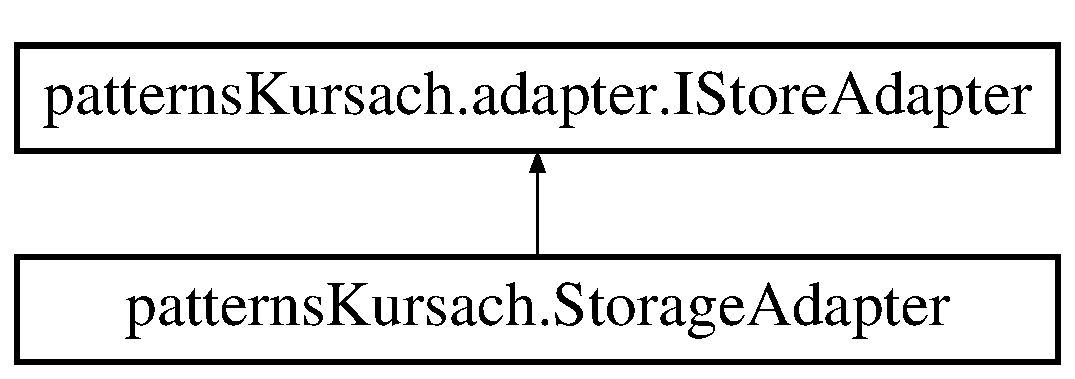
\includegraphics[height=2.000000cm]{interfacepatterns_kursach_1_1adapter_1_1_i_store_adapter}
\end{center}
\end{figure}
\subsection*{Public Member Functions}
\begin{DoxyCompactItemize}
\item 
Data\+Row \mbox{\hyperlink{interfacepatterns_kursach_1_1adapter_1_1_i_store_adapter_a23ec87fad2ed69f4aeb2cc98369dfcc0}{find\+Id}} (int id, String table)
\item 
Data\+Row \mbox{[}$\,$\mbox{]} \mbox{\hyperlink{interfacepatterns_kursach_1_1adapter_1_1_i_store_adapter_a13f0beab6001c24e72b16d3afa1c5f7a}{find\+All}} (String table)
\item 
Data\+Row \mbox{[}$\,$\mbox{]} \mbox{\hyperlink{interfacepatterns_kursach_1_1adapter_1_1_i_store_adapter_aa213143da13c4772d0aa695ece08b3ac}{find\+Side\+Kick}} (String table, String v\+Key, int id)
\item 
void \mbox{\hyperlink{interfacepatterns_kursach_1_1adapter_1_1_i_store_adapter_a68e63038dd5b807330386f8ac774896a}{edit}} (String table, Dictionary$<$ String, Object $>$ colums, int id)
\item 
void \mbox{\hyperlink{interfacepatterns_kursach_1_1adapter_1_1_i_store_adapter_a12816166876b9ddffa991a55d5e917c8}{add}} (String table, List$<$ Object $>$ colums)
\item 
void \mbox{\hyperlink{interfacepatterns_kursach_1_1adapter_1_1_i_store_adapter_a938d47744137644c9da0e8d745823238}{delete}} (String table, int id)
\item 
Data\+Row \mbox{[}$\,$\mbox{]} \mbox{\hyperlink{interfacepatterns_kursach_1_1adapter_1_1_i_store_adapter_a2f461380a248778258d993f8dc1eb265}{sql\+Execute}} (String sql)
\item 
void \mbox{\hyperlink{interfacepatterns_kursach_1_1adapter_1_1_i_store_adapter_ad1833d2efd297547ff34828468e914d2}{Add\+Update\+Execute}} (String sql)
\end{DoxyCompactItemize}


\subsection{Detailed Description}


Definition at line 10 of file I\+Store\+Adapter.\+cs.



\subsection{Member Function Documentation}
\mbox{\Hypertarget{interfacepatterns_kursach_1_1adapter_1_1_i_store_adapter_a12816166876b9ddffa991a55d5e917c8}\label{interfacepatterns_kursach_1_1adapter_1_1_i_store_adapter_a12816166876b9ddffa991a55d5e917c8}} 
\index{patterns\+Kursach\+::adapter\+::\+I\+Store\+Adapter@{patterns\+Kursach\+::adapter\+::\+I\+Store\+Adapter}!add@{add}}
\index{add@{add}!patterns\+Kursach\+::adapter\+::\+I\+Store\+Adapter@{patterns\+Kursach\+::adapter\+::\+I\+Store\+Adapter}}
\subsubsection{\texorpdfstring{add()}{add()}}
{\footnotesize\ttfamily void patterns\+Kursach.\+adapter.\+I\+Store\+Adapter.\+add (\begin{DoxyParamCaption}\item[{String}]{table,  }\item[{List$<$ Object $>$}]{colums }\end{DoxyParamCaption})}



Implemented in \mbox{\hyperlink{classpatterns_kursach_1_1_storage_adapter_a1a6b043621bfa53482563397597aa046}{patterns\+Kursach.\+Storage\+Adapter}}.

\mbox{\Hypertarget{interfacepatterns_kursach_1_1adapter_1_1_i_store_adapter_ad1833d2efd297547ff34828468e914d2}\label{interfacepatterns_kursach_1_1adapter_1_1_i_store_adapter_ad1833d2efd297547ff34828468e914d2}} 
\index{patterns\+Kursach\+::adapter\+::\+I\+Store\+Adapter@{patterns\+Kursach\+::adapter\+::\+I\+Store\+Adapter}!Add\+Update\+Execute@{Add\+Update\+Execute}}
\index{Add\+Update\+Execute@{Add\+Update\+Execute}!patterns\+Kursach\+::adapter\+::\+I\+Store\+Adapter@{patterns\+Kursach\+::adapter\+::\+I\+Store\+Adapter}}
\subsubsection{\texorpdfstring{Add\+Update\+Execute()}{AddUpdateExecute()}}
{\footnotesize\ttfamily void patterns\+Kursach.\+adapter.\+I\+Store\+Adapter.\+Add\+Update\+Execute (\begin{DoxyParamCaption}\item[{String}]{sql }\end{DoxyParamCaption})}



Implemented in \mbox{\hyperlink{classpatterns_kursach_1_1_storage_adapter_a45d79830f42e8ba2341425175559b31b}{patterns\+Kursach.\+Storage\+Adapter}}.

\mbox{\Hypertarget{interfacepatterns_kursach_1_1adapter_1_1_i_store_adapter_a938d47744137644c9da0e8d745823238}\label{interfacepatterns_kursach_1_1adapter_1_1_i_store_adapter_a938d47744137644c9da0e8d745823238}} 
\index{patterns\+Kursach\+::adapter\+::\+I\+Store\+Adapter@{patterns\+Kursach\+::adapter\+::\+I\+Store\+Adapter}!delete@{delete}}
\index{delete@{delete}!patterns\+Kursach\+::adapter\+::\+I\+Store\+Adapter@{patterns\+Kursach\+::adapter\+::\+I\+Store\+Adapter}}
\subsubsection{\texorpdfstring{delete()}{delete()}}
{\footnotesize\ttfamily void patterns\+Kursach.\+adapter.\+I\+Store\+Adapter.\+delete (\begin{DoxyParamCaption}\item[{String}]{table,  }\item[{int}]{id }\end{DoxyParamCaption})}



Implemented in \mbox{\hyperlink{classpatterns_kursach_1_1_storage_adapter_a6c87c580a8bdc3e2803ae31e59ad0071}{patterns\+Kursach.\+Storage\+Adapter}}.

\mbox{\Hypertarget{interfacepatterns_kursach_1_1adapter_1_1_i_store_adapter_a68e63038dd5b807330386f8ac774896a}\label{interfacepatterns_kursach_1_1adapter_1_1_i_store_adapter_a68e63038dd5b807330386f8ac774896a}} 
\index{patterns\+Kursach\+::adapter\+::\+I\+Store\+Adapter@{patterns\+Kursach\+::adapter\+::\+I\+Store\+Adapter}!edit@{edit}}
\index{edit@{edit}!patterns\+Kursach\+::adapter\+::\+I\+Store\+Adapter@{patterns\+Kursach\+::adapter\+::\+I\+Store\+Adapter}}
\subsubsection{\texorpdfstring{edit()}{edit()}}
{\footnotesize\ttfamily void patterns\+Kursach.\+adapter.\+I\+Store\+Adapter.\+edit (\begin{DoxyParamCaption}\item[{String}]{table,  }\item[{Dictionary$<$ String, Object $>$}]{colums,  }\item[{int}]{id }\end{DoxyParamCaption})}



Implemented in \mbox{\hyperlink{classpatterns_kursach_1_1_storage_adapter_abb78e8f3b4afc32f724141fd36cf3bfb}{patterns\+Kursach.\+Storage\+Adapter}}.

\mbox{\Hypertarget{interfacepatterns_kursach_1_1adapter_1_1_i_store_adapter_a13f0beab6001c24e72b16d3afa1c5f7a}\label{interfacepatterns_kursach_1_1adapter_1_1_i_store_adapter_a13f0beab6001c24e72b16d3afa1c5f7a}} 
\index{patterns\+Kursach\+::adapter\+::\+I\+Store\+Adapter@{patterns\+Kursach\+::adapter\+::\+I\+Store\+Adapter}!find\+All@{find\+All}}
\index{find\+All@{find\+All}!patterns\+Kursach\+::adapter\+::\+I\+Store\+Adapter@{patterns\+Kursach\+::adapter\+::\+I\+Store\+Adapter}}
\subsubsection{\texorpdfstring{find\+All()}{findAll()}}
{\footnotesize\ttfamily Data\+Row \mbox{[}$\,$\mbox{]} patterns\+Kursach.\+adapter.\+I\+Store\+Adapter.\+find\+All (\begin{DoxyParamCaption}\item[{String}]{table }\end{DoxyParamCaption})}



Implemented in \mbox{\hyperlink{classpatterns_kursach_1_1_storage_adapter_a08e1b401021fac85dfd2f22a8654171a}{patterns\+Kursach.\+Storage\+Adapter}}.

\mbox{\Hypertarget{interfacepatterns_kursach_1_1adapter_1_1_i_store_adapter_a23ec87fad2ed69f4aeb2cc98369dfcc0}\label{interfacepatterns_kursach_1_1adapter_1_1_i_store_adapter_a23ec87fad2ed69f4aeb2cc98369dfcc0}} 
\index{patterns\+Kursach\+::adapter\+::\+I\+Store\+Adapter@{patterns\+Kursach\+::adapter\+::\+I\+Store\+Adapter}!find\+Id@{find\+Id}}
\index{find\+Id@{find\+Id}!patterns\+Kursach\+::adapter\+::\+I\+Store\+Adapter@{patterns\+Kursach\+::adapter\+::\+I\+Store\+Adapter}}
\subsubsection{\texorpdfstring{find\+Id()}{findId()}}
{\footnotesize\ttfamily Data\+Row patterns\+Kursach.\+adapter.\+I\+Store\+Adapter.\+find\+Id (\begin{DoxyParamCaption}\item[{int}]{id,  }\item[{String}]{table }\end{DoxyParamCaption})}



Implemented in \mbox{\hyperlink{classpatterns_kursach_1_1_storage_adapter_a6b1e7c2a228f04ef4708702a8e11f114}{patterns\+Kursach.\+Storage\+Adapter}}.

\mbox{\Hypertarget{interfacepatterns_kursach_1_1adapter_1_1_i_store_adapter_aa213143da13c4772d0aa695ece08b3ac}\label{interfacepatterns_kursach_1_1adapter_1_1_i_store_adapter_aa213143da13c4772d0aa695ece08b3ac}} 
\index{patterns\+Kursach\+::adapter\+::\+I\+Store\+Adapter@{patterns\+Kursach\+::adapter\+::\+I\+Store\+Adapter}!find\+Side\+Kick@{find\+Side\+Kick}}
\index{find\+Side\+Kick@{find\+Side\+Kick}!patterns\+Kursach\+::adapter\+::\+I\+Store\+Adapter@{patterns\+Kursach\+::adapter\+::\+I\+Store\+Adapter}}
\subsubsection{\texorpdfstring{find\+Side\+Kick()}{findSideKick()}}
{\footnotesize\ttfamily Data\+Row \mbox{[}$\,$\mbox{]} patterns\+Kursach.\+adapter.\+I\+Store\+Adapter.\+find\+Side\+Kick (\begin{DoxyParamCaption}\item[{String}]{table,  }\item[{String}]{v\+Key,  }\item[{int}]{id }\end{DoxyParamCaption})}



Implemented in \mbox{\hyperlink{classpatterns_kursach_1_1_storage_adapter_a25fff62c20799364eebdb38515169fb1}{patterns\+Kursach.\+Storage\+Adapter}}.

\mbox{\Hypertarget{interfacepatterns_kursach_1_1adapter_1_1_i_store_adapter_a2f461380a248778258d993f8dc1eb265}\label{interfacepatterns_kursach_1_1adapter_1_1_i_store_adapter_a2f461380a248778258d993f8dc1eb265}} 
\index{patterns\+Kursach\+::adapter\+::\+I\+Store\+Adapter@{patterns\+Kursach\+::adapter\+::\+I\+Store\+Adapter}!sql\+Execute@{sql\+Execute}}
\index{sql\+Execute@{sql\+Execute}!patterns\+Kursach\+::adapter\+::\+I\+Store\+Adapter@{patterns\+Kursach\+::adapter\+::\+I\+Store\+Adapter}}
\subsubsection{\texorpdfstring{sql\+Execute()}{sqlExecute()}}
{\footnotesize\ttfamily Data\+Row \mbox{[}$\,$\mbox{]} patterns\+Kursach.\+adapter.\+I\+Store\+Adapter.\+sql\+Execute (\begin{DoxyParamCaption}\item[{String}]{sql }\end{DoxyParamCaption})}



Implemented in \mbox{\hyperlink{classpatterns_kursach_1_1_storage_adapter_a6ad39a4e1cc12887ba0f3f8563032c6d}{patterns\+Kursach.\+Storage\+Adapter}}.



The documentation for this interface was generated from the following file\+:\begin{DoxyCompactItemize}
\item 
patterns\+Kursach/\mbox{\hyperlink{_i_store_adapter_8cs}{I\+Store\+Adapter.\+cs}}\end{DoxyCompactItemize}

\hypertarget{classpatterns_kursach_1_1_login}{}\section{patterns\+Kursach.\+Login Class Reference}
\label{classpatterns_kursach_1_1_login}\index{patterns\+Kursach.\+Login@{patterns\+Kursach.\+Login}}
Inheritance diagram for patterns\+Kursach.\+Login\+:\begin{figure}[H]
\begin{center}
\leavevmode
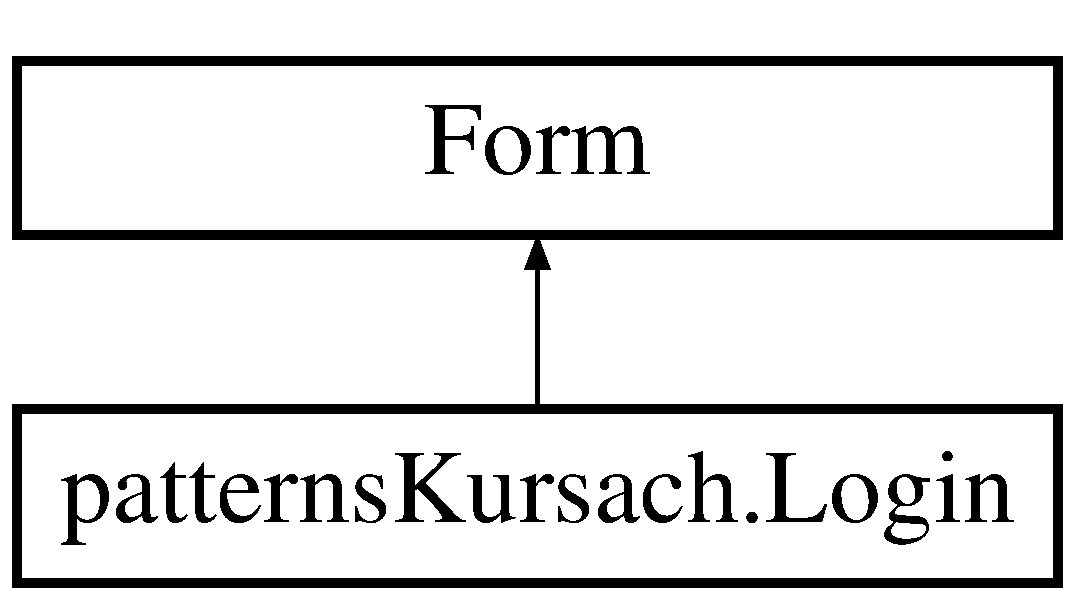
\includegraphics[height=2.000000cm]{classpatterns_kursach_1_1_login}
\end{center}
\end{figure}
\subsection*{Public Member Functions}
\begin{DoxyCompactItemize}
\item 
\mbox{\hyperlink{classpatterns_kursach_1_1_login_a634b6674a8c0c0ceace74f06683b1e2a}{Login}} ()
\end{DoxyCompactItemize}
\subsection*{Protected Member Functions}
\begin{DoxyCompactItemize}
\item 
override void \mbox{\hyperlink{classpatterns_kursach_1_1_login_ad03dba5cc72d1a588166064d049911db}{Dispose}} (bool disposing)
\begin{DoxyCompactList}\small\item\em Освободить все используемые ресурсы. \end{DoxyCompactList}\end{DoxyCompactItemize}


\subsection{Detailed Description}


Definition at line 12 of file Login.\+cs.



\subsection{Constructor \& Destructor Documentation}
\mbox{\Hypertarget{classpatterns_kursach_1_1_login_a634b6674a8c0c0ceace74f06683b1e2a}\label{classpatterns_kursach_1_1_login_a634b6674a8c0c0ceace74f06683b1e2a}} 
\index{patterns\+Kursach\+::\+Login@{patterns\+Kursach\+::\+Login}!Login@{Login}}
\index{Login@{Login}!patterns\+Kursach\+::\+Login@{patterns\+Kursach\+::\+Login}}
\subsubsection{\texorpdfstring{Login()}{Login()}}
{\footnotesize\ttfamily patterns\+Kursach.\+Login.\+Login (\begin{DoxyParamCaption}{ }\end{DoxyParamCaption})}



Definition at line 14 of file Login.\+cs.



\subsection{Member Function Documentation}
\mbox{\Hypertarget{classpatterns_kursach_1_1_login_ad03dba5cc72d1a588166064d049911db}\label{classpatterns_kursach_1_1_login_ad03dba5cc72d1a588166064d049911db}} 
\index{patterns\+Kursach\+::\+Login@{patterns\+Kursach\+::\+Login}!Dispose@{Dispose}}
\index{Dispose@{Dispose}!patterns\+Kursach\+::\+Login@{patterns\+Kursach\+::\+Login}}
\subsubsection{\texorpdfstring{Dispose()}{Dispose()}}
{\footnotesize\ttfamily override void patterns\+Kursach.\+Login.\+Dispose (\begin{DoxyParamCaption}\item[{bool}]{disposing }\end{DoxyParamCaption})\hspace{0.3cm}{\ttfamily [protected]}}



Освободить все используемые ресурсы. 


\begin{DoxyParams}{Parameters}
{\em disposing} & истинно, если управляемый ресурс должен быть удален; иначе ложно.\\
\hline
\end{DoxyParams}


Definition at line 14 of file Login.\+Designer.\+cs.



The documentation for this class was generated from the following files\+:\begin{DoxyCompactItemize}
\item 
patterns\+Kursach/\mbox{\hyperlink{_login_8cs}{Login.\+cs}}\item 
patterns\+Kursach/\mbox{\hyperlink{_login_8_designer_8cs}{Login.\+Designer.\+cs}}\end{DoxyCompactItemize}

\hypertarget{classpatterns_kursach_1_1_metodichka}{}\section{patterns\+Kursach.\+Metodichka Class Reference}
\label{classpatterns_kursach_1_1_metodichka}\index{patterns\+Kursach.\+Metodichka@{patterns\+Kursach.\+Metodichka}}
\subsection*{Public Member Functions}
\begin{DoxyCompactItemize}
\item 
\mbox{\hyperlink{classpatterns_kursach_1_1_metodichka_ae38e404f5ac9b9bbbc015d4303616dbc}{Metodichka}} (int id, string name, string subject, string coauthor)
\item 
\mbox{\hyperlink{classpatterns_kursach_1_1_metodichka_a21bfce8717cc47d75b3b6a102cd2e076}{Metodichka}} (Data\+Row datas)
\end{DoxyCompactItemize}
\subsection*{Properties}
\begin{DoxyCompactItemize}
\item 
int \mbox{\hyperlink{classpatterns_kursach_1_1_metodichka_af1eef999fed5331bd81a0b45e5cbfc10}{Id}}\hspace{0.3cm}{\ttfamily  \mbox{[}get, set\mbox{]}}
\item 
string \mbox{\hyperlink{classpatterns_kursach_1_1_metodichka_a5060cb3a5ac2c9ead4f076e7d7b1528a}{Name}}\hspace{0.3cm}{\ttfamily  \mbox{[}get, set\mbox{]}}
\item 
string \mbox{\hyperlink{classpatterns_kursach_1_1_metodichka_a750ddc05459babd1b2a68a7c18358522}{Subject}}\hspace{0.3cm}{\ttfamily  \mbox{[}get, set\mbox{]}}
\item 
string \mbox{\hyperlink{classpatterns_kursach_1_1_metodichka_a4f93600800bc458da0cb1b1b70d540d4}{Coauthor}}\hspace{0.3cm}{\ttfamily  \mbox{[}get, set\mbox{]}}
\end{DoxyCompactItemize}


\subsection{Detailed Description}


Definition at line 10 of file Metodichka.\+cs.



\subsection{Constructor \& Destructor Documentation}
\mbox{\Hypertarget{classpatterns_kursach_1_1_metodichka_ae38e404f5ac9b9bbbc015d4303616dbc}\label{classpatterns_kursach_1_1_metodichka_ae38e404f5ac9b9bbbc015d4303616dbc}} 
\index{patterns\+Kursach\+::\+Metodichka@{patterns\+Kursach\+::\+Metodichka}!Metodichka@{Metodichka}}
\index{Metodichka@{Metodichka}!patterns\+Kursach\+::\+Metodichka@{patterns\+Kursach\+::\+Metodichka}}
\subsubsection{\texorpdfstring{Metodichka()}{Metodichka()}\hspace{0.1cm}{\footnotesize\ttfamily [1/2]}}
{\footnotesize\ttfamily patterns\+Kursach.\+Metodichka.\+Metodichka (\begin{DoxyParamCaption}\item[{int}]{id,  }\item[{string}]{name,  }\item[{string}]{subject,  }\item[{string}]{coauthor }\end{DoxyParamCaption})}



Definition at line 20 of file Metodichka.\+cs.

\mbox{\Hypertarget{classpatterns_kursach_1_1_metodichka_a21bfce8717cc47d75b3b6a102cd2e076}\label{classpatterns_kursach_1_1_metodichka_a21bfce8717cc47d75b3b6a102cd2e076}} 
\index{patterns\+Kursach\+::\+Metodichka@{patterns\+Kursach\+::\+Metodichka}!Metodichka@{Metodichka}}
\index{Metodichka@{Metodichka}!patterns\+Kursach\+::\+Metodichka@{patterns\+Kursach\+::\+Metodichka}}
\subsubsection{\texorpdfstring{Metodichka()}{Metodichka()}\hspace{0.1cm}{\footnotesize\ttfamily [2/2]}}
{\footnotesize\ttfamily patterns\+Kursach.\+Metodichka.\+Metodichka (\begin{DoxyParamCaption}\item[{Data\+Row}]{datas }\end{DoxyParamCaption})}



Definition at line 33 of file Metodichka.\+cs.



\subsection{Property Documentation}
\mbox{\Hypertarget{classpatterns_kursach_1_1_metodichka_a4f93600800bc458da0cb1b1b70d540d4}\label{classpatterns_kursach_1_1_metodichka_a4f93600800bc458da0cb1b1b70d540d4}} 
\index{patterns\+Kursach\+::\+Metodichka@{patterns\+Kursach\+::\+Metodichka}!Coauthor@{Coauthor}}
\index{Coauthor@{Coauthor}!patterns\+Kursach\+::\+Metodichka@{patterns\+Kursach\+::\+Metodichka}}
\subsubsection{\texorpdfstring{Coauthor}{Coauthor}}
{\footnotesize\ttfamily string patterns\+Kursach.\+Metodichka.\+Coauthor\hspace{0.3cm}{\ttfamily [get]}, {\ttfamily [set]}}



Definition at line 31 of file Metodichka.\+cs.

\mbox{\Hypertarget{classpatterns_kursach_1_1_metodichka_af1eef999fed5331bd81a0b45e5cbfc10}\label{classpatterns_kursach_1_1_metodichka_af1eef999fed5331bd81a0b45e5cbfc10}} 
\index{patterns\+Kursach\+::\+Metodichka@{patterns\+Kursach\+::\+Metodichka}!Id@{Id}}
\index{Id@{Id}!patterns\+Kursach\+::\+Metodichka@{patterns\+Kursach\+::\+Metodichka}}
\subsubsection{\texorpdfstring{Id}{Id}}
{\footnotesize\ttfamily int patterns\+Kursach.\+Metodichka.\+Id\hspace{0.3cm}{\ttfamily [get]}, {\ttfamily [set]}}



Definition at line 28 of file Metodichka.\+cs.

\mbox{\Hypertarget{classpatterns_kursach_1_1_metodichka_a5060cb3a5ac2c9ead4f076e7d7b1528a}\label{classpatterns_kursach_1_1_metodichka_a5060cb3a5ac2c9ead4f076e7d7b1528a}} 
\index{patterns\+Kursach\+::\+Metodichka@{patterns\+Kursach\+::\+Metodichka}!Name@{Name}}
\index{Name@{Name}!patterns\+Kursach\+::\+Metodichka@{patterns\+Kursach\+::\+Metodichka}}
\subsubsection{\texorpdfstring{Name}{Name}}
{\footnotesize\ttfamily string patterns\+Kursach.\+Metodichka.\+Name\hspace{0.3cm}{\ttfamily [get]}, {\ttfamily [set]}}



Definition at line 29 of file Metodichka.\+cs.

\mbox{\Hypertarget{classpatterns_kursach_1_1_metodichka_a750ddc05459babd1b2a68a7c18358522}\label{classpatterns_kursach_1_1_metodichka_a750ddc05459babd1b2a68a7c18358522}} 
\index{patterns\+Kursach\+::\+Metodichka@{patterns\+Kursach\+::\+Metodichka}!Subject@{Subject}}
\index{Subject@{Subject}!patterns\+Kursach\+::\+Metodichka@{patterns\+Kursach\+::\+Metodichka}}
\subsubsection{\texorpdfstring{Subject}{Subject}}
{\footnotesize\ttfamily string patterns\+Kursach.\+Metodichka.\+Subject\hspace{0.3cm}{\ttfamily [get]}, {\ttfamily [set]}}



Definition at line 30 of file Metodichka.\+cs.



The documentation for this class was generated from the following file\+:\begin{DoxyCompactItemize}
\item 
patterns\+Kursach/\mbox{\hyperlink{_metodichka_8cs}{Metodichka.\+cs}}\end{DoxyCompactItemize}

\hypertarget{classpatterns_kursach_1_1_progress}{}\section{patterns\+Kursach.\+Progress Class Reference}
\label{classpatterns_kursach_1_1_progress}\index{patterns\+Kursach.\+Progress@{patterns\+Kursach.\+Progress}}
\subsection*{Public Member Functions}
\begin{DoxyCompactItemize}
\item 
\mbox{\hyperlink{classpatterns_kursach_1_1_progress_a5c6803058985cb88e49a24c9c8816db0}{Progress}} (int id, string name, int position)
\item 
\mbox{\hyperlink{classpatterns_kursach_1_1_progress_abfb0c1805d881ed4a36a08288093ac57}{Progress}} (Data\+Row datas)
\end{DoxyCompactItemize}
\subsection*{Properties}
\begin{DoxyCompactItemize}
\item 
int \mbox{\hyperlink{classpatterns_kursach_1_1_progress_ae639d8ba609612325b731e91a901927a}{Id}}\hspace{0.3cm}{\ttfamily  \mbox{[}get, set\mbox{]}}
\item 
string \mbox{\hyperlink{classpatterns_kursach_1_1_progress_a8f55b8fc822cec0cc2cfb1b9d5c4c535}{Name}}\hspace{0.3cm}{\ttfamily  \mbox{[}get, set\mbox{]}}
\item 
int \mbox{\hyperlink{classpatterns_kursach_1_1_progress_ac6f738598992b81afb7bab6b646e8714}{Position}}\hspace{0.3cm}{\ttfamily  \mbox{[}get, set\mbox{]}}
\end{DoxyCompactItemize}


\subsection{Detailed Description}


Definition at line 10 of file Progress.\+cs.



\subsection{Constructor \& Destructor Documentation}
\mbox{\Hypertarget{classpatterns_kursach_1_1_progress_a5c6803058985cb88e49a24c9c8816db0}\label{classpatterns_kursach_1_1_progress_a5c6803058985cb88e49a24c9c8816db0}} 
\index{patterns\+Kursach\+::\+Progress@{patterns\+Kursach\+::\+Progress}!Progress@{Progress}}
\index{Progress@{Progress}!patterns\+Kursach\+::\+Progress@{patterns\+Kursach\+::\+Progress}}
\subsubsection{\texorpdfstring{Progress()}{Progress()}\hspace{0.1cm}{\footnotesize\ttfamily [1/2]}}
{\footnotesize\ttfamily patterns\+Kursach.\+Progress.\+Progress (\begin{DoxyParamCaption}\item[{int}]{id,  }\item[{string}]{name,  }\item[{int}]{position }\end{DoxyParamCaption})}



Definition at line 18 of file Progress.\+cs.

\mbox{\Hypertarget{classpatterns_kursach_1_1_progress_abfb0c1805d881ed4a36a08288093ac57}\label{classpatterns_kursach_1_1_progress_abfb0c1805d881ed4a36a08288093ac57}} 
\index{patterns\+Kursach\+::\+Progress@{patterns\+Kursach\+::\+Progress}!Progress@{Progress}}
\index{Progress@{Progress}!patterns\+Kursach\+::\+Progress@{patterns\+Kursach\+::\+Progress}}
\subsubsection{\texorpdfstring{Progress()}{Progress()}\hspace{0.1cm}{\footnotesize\ttfamily [2/2]}}
{\footnotesize\ttfamily patterns\+Kursach.\+Progress.\+Progress (\begin{DoxyParamCaption}\item[{Data\+Row}]{datas }\end{DoxyParamCaption})}



Definition at line 29 of file Progress.\+cs.



\subsection{Property Documentation}
\mbox{\Hypertarget{classpatterns_kursach_1_1_progress_ae639d8ba609612325b731e91a901927a}\label{classpatterns_kursach_1_1_progress_ae639d8ba609612325b731e91a901927a}} 
\index{patterns\+Kursach\+::\+Progress@{patterns\+Kursach\+::\+Progress}!Id@{Id}}
\index{Id@{Id}!patterns\+Kursach\+::\+Progress@{patterns\+Kursach\+::\+Progress}}
\subsubsection{\texorpdfstring{Id}{Id}}
{\footnotesize\ttfamily int patterns\+Kursach.\+Progress.\+Id\hspace{0.3cm}{\ttfamily [get]}, {\ttfamily [set]}}



Definition at line 25 of file Progress.\+cs.

\mbox{\Hypertarget{classpatterns_kursach_1_1_progress_a8f55b8fc822cec0cc2cfb1b9d5c4c535}\label{classpatterns_kursach_1_1_progress_a8f55b8fc822cec0cc2cfb1b9d5c4c535}} 
\index{patterns\+Kursach\+::\+Progress@{patterns\+Kursach\+::\+Progress}!Name@{Name}}
\index{Name@{Name}!patterns\+Kursach\+::\+Progress@{patterns\+Kursach\+::\+Progress}}
\subsubsection{\texorpdfstring{Name}{Name}}
{\footnotesize\ttfamily string patterns\+Kursach.\+Progress.\+Name\hspace{0.3cm}{\ttfamily [get]}, {\ttfamily [set]}}



Definition at line 26 of file Progress.\+cs.

\mbox{\Hypertarget{classpatterns_kursach_1_1_progress_ac6f738598992b81afb7bab6b646e8714}\label{classpatterns_kursach_1_1_progress_ac6f738598992b81afb7bab6b646e8714}} 
\index{patterns\+Kursach\+::\+Progress@{patterns\+Kursach\+::\+Progress}!Position@{Position}}
\index{Position@{Position}!patterns\+Kursach\+::\+Progress@{patterns\+Kursach\+::\+Progress}}
\subsubsection{\texorpdfstring{Position}{Position}}
{\footnotesize\ttfamily int patterns\+Kursach.\+Progress.\+Position\hspace{0.3cm}{\ttfamily [get]}, {\ttfamily [set]}}



Definition at line 27 of file Progress.\+cs.



The documentation for this class was generated from the following file\+:\begin{DoxyCompactItemize}
\item 
patterns\+Kursach/\mbox{\hyperlink{_progress_8cs}{Progress.\+cs}}\end{DoxyCompactItemize}

\hypertarget{classpatterns_kursach_1_1_publish}{}\section{patterns\+Kursach.\+Publish Class Reference}
\label{classpatterns_kursach_1_1_publish}\index{patterns\+Kursach.\+Publish@{patterns\+Kursach.\+Publish}}
\subsection*{Public Member Functions}
\begin{DoxyCompactItemize}
\item 
\mbox{\hyperlink{classpatterns_kursach_1_1_publish_a24b11257b2dc624f57ae7a54c6f2b4df}{Publish}} (int id, string tema, string place)
\item 
\mbox{\hyperlink{classpatterns_kursach_1_1_publish_aa4276c74c450ea5d52ad3c5d993957e7}{Publish}} (Data\+Row datas)
\end{DoxyCompactItemize}
\subsection*{Properties}
\begin{DoxyCompactItemize}
\item 
int \mbox{\hyperlink{classpatterns_kursach_1_1_publish_aea975a97fda5fe5ce6819b39f44dea76}{Id}}\hspace{0.3cm}{\ttfamily  \mbox{[}get, set\mbox{]}}
\item 
string \mbox{\hyperlink{classpatterns_kursach_1_1_publish_a0e90f8e6a65fb7af38629af11f9df0fc}{Tema}}\hspace{0.3cm}{\ttfamily  \mbox{[}get, set\mbox{]}}
\item 
string \mbox{\hyperlink{classpatterns_kursach_1_1_publish_ac20d4f17cd986d842eb5840f121fcec6}{Place}}\hspace{0.3cm}{\ttfamily  \mbox{[}get, set\mbox{]}}
\end{DoxyCompactItemize}


\subsection{Detailed Description}


Definition at line 10 of file Publish.\+cs.



\subsection{Constructor \& Destructor Documentation}
\mbox{\Hypertarget{classpatterns_kursach_1_1_publish_a24b11257b2dc624f57ae7a54c6f2b4df}\label{classpatterns_kursach_1_1_publish_a24b11257b2dc624f57ae7a54c6f2b4df}} 
\index{patterns\+Kursach\+::\+Publish@{patterns\+Kursach\+::\+Publish}!Publish@{Publish}}
\index{Publish@{Publish}!patterns\+Kursach\+::\+Publish@{patterns\+Kursach\+::\+Publish}}
\subsubsection{\texorpdfstring{Publish()}{Publish()}\hspace{0.1cm}{\footnotesize\ttfamily [1/2]}}
{\footnotesize\ttfamily patterns\+Kursach.\+Publish.\+Publish (\begin{DoxyParamCaption}\item[{int}]{id,  }\item[{string}]{tema,  }\item[{string}]{place }\end{DoxyParamCaption})}



Definition at line 18 of file Publish.\+cs.

\mbox{\Hypertarget{classpatterns_kursach_1_1_publish_aa4276c74c450ea5d52ad3c5d993957e7}\label{classpatterns_kursach_1_1_publish_aa4276c74c450ea5d52ad3c5d993957e7}} 
\index{patterns\+Kursach\+::\+Publish@{patterns\+Kursach\+::\+Publish}!Publish@{Publish}}
\index{Publish@{Publish}!patterns\+Kursach\+::\+Publish@{patterns\+Kursach\+::\+Publish}}
\subsubsection{\texorpdfstring{Publish()}{Publish()}\hspace{0.1cm}{\footnotesize\ttfamily [2/2]}}
{\footnotesize\ttfamily patterns\+Kursach.\+Publish.\+Publish (\begin{DoxyParamCaption}\item[{Data\+Row}]{datas }\end{DoxyParamCaption})}



Definition at line 29 of file Publish.\+cs.



\subsection{Property Documentation}
\mbox{\Hypertarget{classpatterns_kursach_1_1_publish_aea975a97fda5fe5ce6819b39f44dea76}\label{classpatterns_kursach_1_1_publish_aea975a97fda5fe5ce6819b39f44dea76}} 
\index{patterns\+Kursach\+::\+Publish@{patterns\+Kursach\+::\+Publish}!Id@{Id}}
\index{Id@{Id}!patterns\+Kursach\+::\+Publish@{patterns\+Kursach\+::\+Publish}}
\subsubsection{\texorpdfstring{Id}{Id}}
{\footnotesize\ttfamily int patterns\+Kursach.\+Publish.\+Id\hspace{0.3cm}{\ttfamily [get]}, {\ttfamily [set]}}



Definition at line 25 of file Publish.\+cs.

\mbox{\Hypertarget{classpatterns_kursach_1_1_publish_ac20d4f17cd986d842eb5840f121fcec6}\label{classpatterns_kursach_1_1_publish_ac20d4f17cd986d842eb5840f121fcec6}} 
\index{patterns\+Kursach\+::\+Publish@{patterns\+Kursach\+::\+Publish}!Place@{Place}}
\index{Place@{Place}!patterns\+Kursach\+::\+Publish@{patterns\+Kursach\+::\+Publish}}
\subsubsection{\texorpdfstring{Place}{Place}}
{\footnotesize\ttfamily string patterns\+Kursach.\+Publish.\+Place\hspace{0.3cm}{\ttfamily [get]}, {\ttfamily [set]}}



Definition at line 27 of file Publish.\+cs.

\mbox{\Hypertarget{classpatterns_kursach_1_1_publish_a0e90f8e6a65fb7af38629af11f9df0fc}\label{classpatterns_kursach_1_1_publish_a0e90f8e6a65fb7af38629af11f9df0fc}} 
\index{patterns\+Kursach\+::\+Publish@{patterns\+Kursach\+::\+Publish}!Tema@{Tema}}
\index{Tema@{Tema}!patterns\+Kursach\+::\+Publish@{patterns\+Kursach\+::\+Publish}}
\subsubsection{\texorpdfstring{Tema}{Tema}}
{\footnotesize\ttfamily string patterns\+Kursach.\+Publish.\+Tema\hspace{0.3cm}{\ttfamily [get]}, {\ttfamily [set]}}



Definition at line 26 of file Publish.\+cs.



The documentation for this class was generated from the following file\+:\begin{DoxyCompactItemize}
\item 
patterns\+Kursach/\mbox{\hyperlink{_publish_8cs}{Publish.\+cs}}\end{DoxyCompactItemize}

\hypertarget{classpatterns_kursach_1_1_storage_adapter}{}\section{patterns\+Kursach.\+Storage\+Adapter Class Reference}
\label{classpatterns_kursach_1_1_storage_adapter}\index{patterns\+Kursach.\+Storage\+Adapter@{patterns\+Kursach.\+Storage\+Adapter}}
Inheritance diagram for patterns\+Kursach.\+Storage\+Adapter\+:\begin{figure}[H]
\begin{center}
\leavevmode
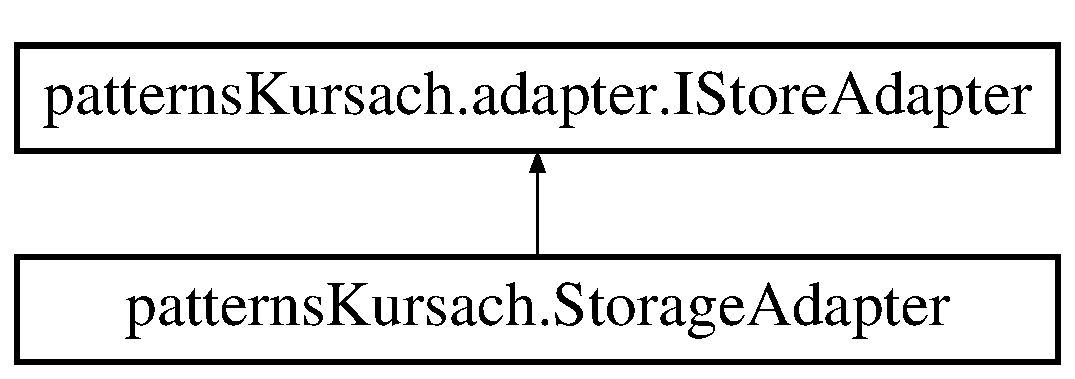
\includegraphics[height=2.000000cm]{classpatterns_kursach_1_1_storage_adapter}
\end{center}
\end{figure}
\subsection*{Public Member Functions}
\begin{DoxyCompactItemize}
\item 
Data\+Row \mbox{\hyperlink{classpatterns_kursach_1_1_storage_adapter_a6b1e7c2a228f04ef4708702a8e11f114}{find\+Id}} (int id, String table)
\begin{DoxyCompactList}\small\item\em Поиск записи по id \end{DoxyCompactList}\item 
Data\+Row \mbox{[}$\,$\mbox{]} \mbox{\hyperlink{classpatterns_kursach_1_1_storage_adapter_a08e1b401021fac85dfd2f22a8654171a}{find\+All}} (String table)
\begin{DoxyCompactList}\small\item\em Вывод всех данных из таблицы \end{DoxyCompactList}\item 
Data\+Row \mbox{[}$\,$\mbox{]} \mbox{\hyperlink{classpatterns_kursach_1_1_storage_adapter_a25fff62c20799364eebdb38515169fb1}{find\+Side\+Kick}} (String table, String v\+Key, int id)
\begin{DoxyCompactList}\small\item\em Вывод данных из связаной таблицы \end{DoxyCompactList}\item 
void \mbox{\hyperlink{classpatterns_kursach_1_1_storage_adapter_abb78e8f3b4afc32f724141fd36cf3bfb}{edit}} (String table, Dictionary$<$ String, Object $>$ colums, int id)
\begin{DoxyCompactList}\small\item\em Редактирование записи \end{DoxyCompactList}\item 
void \mbox{\hyperlink{classpatterns_kursach_1_1_storage_adapter_a1a6b043621bfa53482563397597aa046}{add}} (String table, List$<$ Object $>$ colums)
\begin{DoxyCompactList}\small\item\em Добавление записи \end{DoxyCompactList}\item 
void \mbox{\hyperlink{classpatterns_kursach_1_1_storage_adapter_a6c87c580a8bdc3e2803ae31e59ad0071}{delete}} (String table, int id)
\begin{DoxyCompactList}\small\item\em Удаление зщаписи \end{DoxyCompactList}\item 
Data\+Row \mbox{[}$\,$\mbox{]} \mbox{\hyperlink{classpatterns_kursach_1_1_storage_adapter_a6ad39a4e1cc12887ba0f3f8563032c6d}{sql\+Execute}} (String sql)
\begin{DoxyCompactList}\small\item\em Выполнение sql скрипта для вывода данных \end{DoxyCompactList}\item 
void \mbox{\hyperlink{classpatterns_kursach_1_1_storage_adapter_a45d79830f42e8ba2341425175559b31b}{Add\+Update\+Execute}} (String sql)
\begin{DoxyCompactList}\small\item\em Выполнение sql скрипта для добавление/обновления данных \end{DoxyCompactList}\end{DoxyCompactItemize}


\subsection{Detailed Description}


Definition at line 11 of file Storage\+Adapter.\+cs.



\subsection{Member Function Documentation}
\mbox{\Hypertarget{classpatterns_kursach_1_1_storage_adapter_a1a6b043621bfa53482563397597aa046}\label{classpatterns_kursach_1_1_storage_adapter_a1a6b043621bfa53482563397597aa046}} 
\index{patterns\+Kursach\+::\+Storage\+Adapter@{patterns\+Kursach\+::\+Storage\+Adapter}!add@{add}}
\index{add@{add}!patterns\+Kursach\+::\+Storage\+Adapter@{patterns\+Kursach\+::\+Storage\+Adapter}}
\subsubsection{\texorpdfstring{add()}{add()}}
{\footnotesize\ttfamily void patterns\+Kursach.\+Storage\+Adapter.\+add (\begin{DoxyParamCaption}\item[{String}]{table,  }\item[{List$<$ Object $>$}]{colums }\end{DoxyParamCaption})}



Добавление записи 


\begin{DoxyParams}{Parameters}
{\em table} & название таблицы\\
\hline
{\em colums} & Поля\\
\hline
\end{DoxyParams}


Implements \mbox{\hyperlink{interfacepatterns_kursach_1_1adapter_1_1_i_store_adapter_a12816166876b9ddffa991a55d5e917c8}{patterns\+Kursach.\+adapter.\+I\+Store\+Adapter}}.



Definition at line 86 of file Storage\+Adapter.\+cs.

\mbox{\Hypertarget{classpatterns_kursach_1_1_storage_adapter_a45d79830f42e8ba2341425175559b31b}\label{classpatterns_kursach_1_1_storage_adapter_a45d79830f42e8ba2341425175559b31b}} 
\index{patterns\+Kursach\+::\+Storage\+Adapter@{patterns\+Kursach\+::\+Storage\+Adapter}!Add\+Update\+Execute@{Add\+Update\+Execute}}
\index{Add\+Update\+Execute@{Add\+Update\+Execute}!patterns\+Kursach\+::\+Storage\+Adapter@{patterns\+Kursach\+::\+Storage\+Adapter}}
\subsubsection{\texorpdfstring{Add\+Update\+Execute()}{AddUpdateExecute()}}
{\footnotesize\ttfamily void patterns\+Kursach.\+Storage\+Adapter.\+Add\+Update\+Execute (\begin{DoxyParamCaption}\item[{String}]{sql }\end{DoxyParamCaption})}



Выполнение sql скрипта для добавление/обновления данных 


\begin{DoxyParams}{Parameters}
{\em sql} & скрипт\\
\hline
\end{DoxyParams}


Implements \mbox{\hyperlink{interfacepatterns_kursach_1_1adapter_1_1_i_store_adapter_ad1833d2efd297547ff34828468e914d2}{patterns\+Kursach.\+adapter.\+I\+Store\+Adapter}}.



Definition at line 139 of file Storage\+Adapter.\+cs.

\mbox{\Hypertarget{classpatterns_kursach_1_1_storage_adapter_a6c87c580a8bdc3e2803ae31e59ad0071}\label{classpatterns_kursach_1_1_storage_adapter_a6c87c580a8bdc3e2803ae31e59ad0071}} 
\index{patterns\+Kursach\+::\+Storage\+Adapter@{patterns\+Kursach\+::\+Storage\+Adapter}!delete@{delete}}
\index{delete@{delete}!patterns\+Kursach\+::\+Storage\+Adapter@{patterns\+Kursach\+::\+Storage\+Adapter}}
\subsubsection{\texorpdfstring{delete()}{delete()}}
{\footnotesize\ttfamily void patterns\+Kursach.\+Storage\+Adapter.\+delete (\begin{DoxyParamCaption}\item[{String}]{table,  }\item[{int}]{id }\end{DoxyParamCaption})}



Удаление зщаписи 


\begin{DoxyParams}{Parameters}
{\em table} & Название таблицы\\
\hline
{\em id} & id записи\\
\hline
\end{DoxyParams}


Implements \mbox{\hyperlink{interfacepatterns_kursach_1_1adapter_1_1_i_store_adapter_a938d47744137644c9da0e8d745823238}{patterns\+Kursach.\+adapter.\+I\+Store\+Adapter}}.



Definition at line 109 of file Storage\+Adapter.\+cs.

\mbox{\Hypertarget{classpatterns_kursach_1_1_storage_adapter_abb78e8f3b4afc32f724141fd36cf3bfb}\label{classpatterns_kursach_1_1_storage_adapter_abb78e8f3b4afc32f724141fd36cf3bfb}} 
\index{patterns\+Kursach\+::\+Storage\+Adapter@{patterns\+Kursach\+::\+Storage\+Adapter}!edit@{edit}}
\index{edit@{edit}!patterns\+Kursach\+::\+Storage\+Adapter@{patterns\+Kursach\+::\+Storage\+Adapter}}
\subsubsection{\texorpdfstring{edit()}{edit()}}
{\footnotesize\ttfamily void patterns\+Kursach.\+Storage\+Adapter.\+edit (\begin{DoxyParamCaption}\item[{String}]{table,  }\item[{Dictionary$<$ String, Object $>$}]{colums,  }\item[{int}]{id }\end{DoxyParamCaption})}



Редактирование записи 


\begin{DoxyParams}{Parameters}
{\em table} & Название таблицы\\
\hline
{\em colums} & Словарь название поля -\/ значение поля \\
\hline
{\em id} & id записи\\
\hline
\end{DoxyParams}


Implements \mbox{\hyperlink{interfacepatterns_kursach_1_1adapter_1_1_i_store_adapter_a68e63038dd5b807330386f8ac774896a}{patterns\+Kursach.\+adapter.\+I\+Store\+Adapter}}.



Definition at line 58 of file Storage\+Adapter.\+cs.

\mbox{\Hypertarget{classpatterns_kursach_1_1_storage_adapter_a08e1b401021fac85dfd2f22a8654171a}\label{classpatterns_kursach_1_1_storage_adapter_a08e1b401021fac85dfd2f22a8654171a}} 
\index{patterns\+Kursach\+::\+Storage\+Adapter@{patterns\+Kursach\+::\+Storage\+Adapter}!find\+All@{find\+All}}
\index{find\+All@{find\+All}!patterns\+Kursach\+::\+Storage\+Adapter@{patterns\+Kursach\+::\+Storage\+Adapter}}
\subsubsection{\texorpdfstring{find\+All()}{findAll()}}
{\footnotesize\ttfamily Data\+Row \mbox{[}$\,$\mbox{]} patterns\+Kursach.\+Storage\+Adapter.\+find\+All (\begin{DoxyParamCaption}\item[{String}]{table }\end{DoxyParamCaption})}



Вывод всех данных из таблицы 


\begin{DoxyParams}{Parameters}
{\em table} & название таблицы\\
\hline
\end{DoxyParams}
\begin{DoxyReturn}{Returns}
Список данных
\end{DoxyReturn}


Implements \mbox{\hyperlink{interfacepatterns_kursach_1_1adapter_1_1_i_store_adapter_a13f0beab6001c24e72b16d3afa1c5f7a}{patterns\+Kursach.\+adapter.\+I\+Store\+Adapter}}.



Definition at line 33 of file Storage\+Adapter.\+cs.

\mbox{\Hypertarget{classpatterns_kursach_1_1_storage_adapter_a6b1e7c2a228f04ef4708702a8e11f114}\label{classpatterns_kursach_1_1_storage_adapter_a6b1e7c2a228f04ef4708702a8e11f114}} 
\index{patterns\+Kursach\+::\+Storage\+Adapter@{patterns\+Kursach\+::\+Storage\+Adapter}!find\+Id@{find\+Id}}
\index{find\+Id@{find\+Id}!patterns\+Kursach\+::\+Storage\+Adapter@{patterns\+Kursach\+::\+Storage\+Adapter}}
\subsubsection{\texorpdfstring{find\+Id()}{findId()}}
{\footnotesize\ttfamily Data\+Row patterns\+Kursach.\+Storage\+Adapter.\+find\+Id (\begin{DoxyParamCaption}\item[{int}]{id,  }\item[{String}]{table }\end{DoxyParamCaption})}



Поиск записи по id 


\begin{DoxyParams}{Parameters}
{\em id} & id записи\\
\hline
{\em table} & Название таблицы\\
\hline
\end{DoxyParams}
\begin{DoxyReturn}{Returns}
Запись
\end{DoxyReturn}


Implements \mbox{\hyperlink{interfacepatterns_kursach_1_1adapter_1_1_i_store_adapter_a23ec87fad2ed69f4aeb2cc98369dfcc0}{patterns\+Kursach.\+adapter.\+I\+Store\+Adapter}}.



Definition at line 22 of file Storage\+Adapter.\+cs.

\mbox{\Hypertarget{classpatterns_kursach_1_1_storage_adapter_a25fff62c20799364eebdb38515169fb1}\label{classpatterns_kursach_1_1_storage_adapter_a25fff62c20799364eebdb38515169fb1}} 
\index{patterns\+Kursach\+::\+Storage\+Adapter@{patterns\+Kursach\+::\+Storage\+Adapter}!find\+Side\+Kick@{find\+Side\+Kick}}
\index{find\+Side\+Kick@{find\+Side\+Kick}!patterns\+Kursach\+::\+Storage\+Adapter@{patterns\+Kursach\+::\+Storage\+Adapter}}
\subsubsection{\texorpdfstring{find\+Side\+Kick()}{findSideKick()}}
{\footnotesize\ttfamily Data\+Row \mbox{[}$\,$\mbox{]} patterns\+Kursach.\+Storage\+Adapter.\+find\+Side\+Kick (\begin{DoxyParamCaption}\item[{String}]{table,  }\item[{String}]{v\+Key,  }\item[{int}]{id }\end{DoxyParamCaption})}



Вывод данных из связаной таблицы 


\begin{DoxyParams}{Parameters}
{\em table} & название таблицы\\
\hline
{\em v\+Key} & название внешнего ключа\\
\hline
{\em id} & id записи\\
\hline
\end{DoxyParams}
\begin{DoxyReturn}{Returns}
Список данных
\end{DoxyReturn}


Implements \mbox{\hyperlink{interfacepatterns_kursach_1_1adapter_1_1_i_store_adapter_aa213143da13c4772d0aa695ece08b3ac}{patterns\+Kursach.\+adapter.\+I\+Store\+Adapter}}.



Definition at line 46 of file Storage\+Adapter.\+cs.

\mbox{\Hypertarget{classpatterns_kursach_1_1_storage_adapter_a6ad39a4e1cc12887ba0f3f8563032c6d}\label{classpatterns_kursach_1_1_storage_adapter_a6ad39a4e1cc12887ba0f3f8563032c6d}} 
\index{patterns\+Kursach\+::\+Storage\+Adapter@{patterns\+Kursach\+::\+Storage\+Adapter}!sql\+Execute@{sql\+Execute}}
\index{sql\+Execute@{sql\+Execute}!patterns\+Kursach\+::\+Storage\+Adapter@{patterns\+Kursach\+::\+Storage\+Adapter}}
\subsubsection{\texorpdfstring{sql\+Execute()}{sqlExecute()}}
{\footnotesize\ttfamily Data\+Row \mbox{[}$\,$\mbox{]} patterns\+Kursach.\+Storage\+Adapter.\+sql\+Execute (\begin{DoxyParamCaption}\item[{String}]{sql }\end{DoxyParamCaption})}



Выполнение sql скрипта для вывода данных 


\begin{DoxyParams}{Parameters}
{\em sql} & sql скрипт\\
\hline
\end{DoxyParams}
\begin{DoxyReturn}{Returns}

\end{DoxyReturn}


Implements \mbox{\hyperlink{interfacepatterns_kursach_1_1adapter_1_1_i_store_adapter_a2f461380a248778258d993f8dc1eb265}{patterns\+Kursach.\+adapter.\+I\+Store\+Adapter}}.



Definition at line 120 of file Storage\+Adapter.\+cs.



The documentation for this class was generated from the following file\+:\begin{DoxyCompactItemize}
\item 
patterns\+Kursach/\mbox{\hyperlink{_storage_adapter_8cs}{Storage\+Adapter.\+cs}}\end{DoxyCompactItemize}

\hypertarget{classpatterns_kursach_1_1_student}{}\section{patterns\+Kursach.\+Student Class Reference}
\label{classpatterns_kursach_1_1_student}\index{patterns\+Kursach.\+Student@{patterns\+Kursach.\+Student}}
\subsection*{Public Member Functions}
\begin{DoxyCompactItemize}
\item 
\mbox{\hyperlink{classpatterns_kursach_1_1_student_ab7bf302da763ef12015e8943ec233c7c}{Student}} (int id, string name, string spec, string stepen)
\item 
\mbox{\hyperlink{classpatterns_kursach_1_1_student_aa012a5120419833a128fafb8a8755c6b}{Student}} (Data\+Row datas)
\item 
\mbox{\hyperlink{classpatterns_kursach_1_1_student_a597e81962cbb7e16d391e515a07e1df6}{Student}} ()
\end{DoxyCompactItemize}
\subsection*{Properties}
\begin{DoxyCompactItemize}
\item 
string \mbox{\hyperlink{classpatterns_kursach_1_1_student_aaf96519bff25150a3ea2304c22f1cd40}{Spec}}\hspace{0.3cm}{\ttfamily  \mbox{[}get, set\mbox{]}}
\item 
string \mbox{\hyperlink{classpatterns_kursach_1_1_student_abbd331b9b1f5542c08434487e2dcac81}{Name}}\hspace{0.3cm}{\ttfamily  \mbox{[}get, set\mbox{]}}
\item 
string \mbox{\hyperlink{classpatterns_kursach_1_1_student_ac1d80f7fe47b9814382d25f416f68192}{Stepen}}\hspace{0.3cm}{\ttfamily  \mbox{[}get, set\mbox{]}}
\item 
int \mbox{\hyperlink{classpatterns_kursach_1_1_student_a8c20b8105aa12679f00252f5f6009ae6}{Id}}\hspace{0.3cm}{\ttfamily  \mbox{[}get, set\mbox{]}}
\end{DoxyCompactItemize}


\subsection{Detailed Description}


Definition at line 10 of file Student.\+cs.



\subsection{Constructor \& Destructor Documentation}
\mbox{\Hypertarget{classpatterns_kursach_1_1_student_ab7bf302da763ef12015e8943ec233c7c}\label{classpatterns_kursach_1_1_student_ab7bf302da763ef12015e8943ec233c7c}} 
\index{patterns\+Kursach\+::\+Student@{patterns\+Kursach\+::\+Student}!Student@{Student}}
\index{Student@{Student}!patterns\+Kursach\+::\+Student@{patterns\+Kursach\+::\+Student}}
\subsubsection{\texorpdfstring{Student()}{Student()}\hspace{0.1cm}{\footnotesize\ttfamily [1/3]}}
{\footnotesize\ttfamily patterns\+Kursach.\+Student.\+Student (\begin{DoxyParamCaption}\item[{int}]{id,  }\item[{string}]{name,  }\item[{string}]{spec,  }\item[{string}]{stepen }\end{DoxyParamCaption})}



Definition at line 20 of file Student.\+cs.

\mbox{\Hypertarget{classpatterns_kursach_1_1_student_aa012a5120419833a128fafb8a8755c6b}\label{classpatterns_kursach_1_1_student_aa012a5120419833a128fafb8a8755c6b}} 
\index{patterns\+Kursach\+::\+Student@{patterns\+Kursach\+::\+Student}!Student@{Student}}
\index{Student@{Student}!patterns\+Kursach\+::\+Student@{patterns\+Kursach\+::\+Student}}
\subsubsection{\texorpdfstring{Student()}{Student()}\hspace{0.1cm}{\footnotesize\ttfamily [2/3]}}
{\footnotesize\ttfamily patterns\+Kursach.\+Student.\+Student (\begin{DoxyParamCaption}\item[{Data\+Row}]{datas }\end{DoxyParamCaption})}



Definition at line 33 of file Student.\+cs.

\mbox{\Hypertarget{classpatterns_kursach_1_1_student_a597e81962cbb7e16d391e515a07e1df6}\label{classpatterns_kursach_1_1_student_a597e81962cbb7e16d391e515a07e1df6}} 
\index{patterns\+Kursach\+::\+Student@{patterns\+Kursach\+::\+Student}!Student@{Student}}
\index{Student@{Student}!patterns\+Kursach\+::\+Student@{patterns\+Kursach\+::\+Student}}
\subsubsection{\texorpdfstring{Student()}{Student()}\hspace{0.1cm}{\footnotesize\ttfamily [3/3]}}
{\footnotesize\ttfamily patterns\+Kursach.\+Student.\+Student (\begin{DoxyParamCaption}{ }\end{DoxyParamCaption})}



Definition at line 41 of file Student.\+cs.



\subsection{Property Documentation}
\mbox{\Hypertarget{classpatterns_kursach_1_1_student_a8c20b8105aa12679f00252f5f6009ae6}\label{classpatterns_kursach_1_1_student_a8c20b8105aa12679f00252f5f6009ae6}} 
\index{patterns\+Kursach\+::\+Student@{patterns\+Kursach\+::\+Student}!Id@{Id}}
\index{Id@{Id}!patterns\+Kursach\+::\+Student@{patterns\+Kursach\+::\+Student}}
\subsubsection{\texorpdfstring{Id}{Id}}
{\footnotesize\ttfamily int patterns\+Kursach.\+Student.\+Id\hspace{0.3cm}{\ttfamily [get]}, {\ttfamily [set]}}



Definition at line 31 of file Student.\+cs.

\mbox{\Hypertarget{classpatterns_kursach_1_1_student_abbd331b9b1f5542c08434487e2dcac81}\label{classpatterns_kursach_1_1_student_abbd331b9b1f5542c08434487e2dcac81}} 
\index{patterns\+Kursach\+::\+Student@{patterns\+Kursach\+::\+Student}!Name@{Name}}
\index{Name@{Name}!patterns\+Kursach\+::\+Student@{patterns\+Kursach\+::\+Student}}
\subsubsection{\texorpdfstring{Name}{Name}}
{\footnotesize\ttfamily string patterns\+Kursach.\+Student.\+Name\hspace{0.3cm}{\ttfamily [get]}, {\ttfamily [set]}}



Definition at line 29 of file Student.\+cs.

\mbox{\Hypertarget{classpatterns_kursach_1_1_student_aaf96519bff25150a3ea2304c22f1cd40}\label{classpatterns_kursach_1_1_student_aaf96519bff25150a3ea2304c22f1cd40}} 
\index{patterns\+Kursach\+::\+Student@{patterns\+Kursach\+::\+Student}!Spec@{Spec}}
\index{Spec@{Spec}!patterns\+Kursach\+::\+Student@{patterns\+Kursach\+::\+Student}}
\subsubsection{\texorpdfstring{Spec}{Spec}}
{\footnotesize\ttfamily string patterns\+Kursach.\+Student.\+Spec\hspace{0.3cm}{\ttfamily [get]}, {\ttfamily [set]}}



Definition at line 28 of file Student.\+cs.

\mbox{\Hypertarget{classpatterns_kursach_1_1_student_ac1d80f7fe47b9814382d25f416f68192}\label{classpatterns_kursach_1_1_student_ac1d80f7fe47b9814382d25f416f68192}} 
\index{patterns\+Kursach\+::\+Student@{patterns\+Kursach\+::\+Student}!Stepen@{Stepen}}
\index{Stepen@{Stepen}!patterns\+Kursach\+::\+Student@{patterns\+Kursach\+::\+Student}}
\subsubsection{\texorpdfstring{Stepen}{Stepen}}
{\footnotesize\ttfamily string patterns\+Kursach.\+Student.\+Stepen\hspace{0.3cm}{\ttfamily [get]}, {\ttfamily [set]}}



Definition at line 30 of file Student.\+cs.



The documentation for this class was generated from the following file\+:\begin{DoxyCompactItemize}
\item 
patterns\+Kursach/\mbox{\hyperlink{_student_8cs}{Student.\+cs}}\end{DoxyCompactItemize}

\hypertarget{classpatterns_kursach_1_1student}{}\section{patterns\+Kursach.\+student Class Reference}
\label{classpatterns_kursach_1_1student}\index{patterns\+Kursach.\+student@{patterns\+Kursach.\+student}}
Inheritance diagram for patterns\+Kursach.\+student\+:\begin{figure}[H]
\begin{center}
\leavevmode
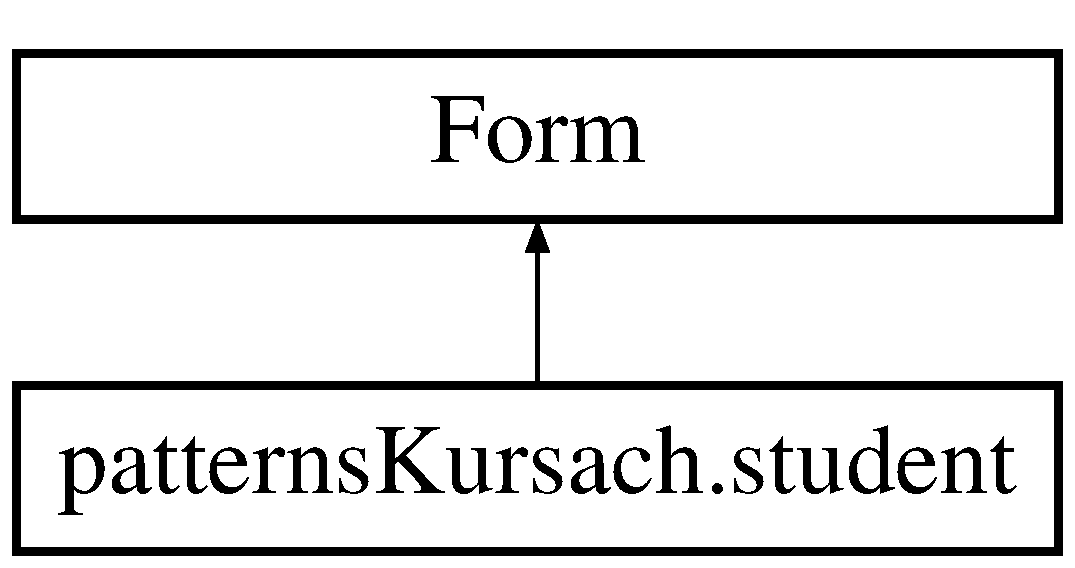
\includegraphics[height=2.000000cm]{classpatterns_kursach_1_1student}
\end{center}
\end{figure}
\subsection*{Public Member Functions}
\begin{DoxyCompactItemize}
\item 
\mbox{\hyperlink{classpatterns_kursach_1_1student_abd0837e0e333877deea0dd7fc79af488}{student}} ()
\item 
void \mbox{\hyperlink{classpatterns_kursach_1_1student_a30dbbf1f0706e7dbac498e79ee42596a}{Fill\+Student}} ()
\item 
void \mbox{\hyperlink{classpatterns_kursach_1_1student_ade5ff561a25e758c638244eeb3777f4d}{Fill\+Attestation}} (int id)
\item 
void \mbox{\hyperlink{classpatterns_kursach_1_1student_ae1bf1deff88ed100f318f8902739abd4}{Fill\+Progress}} (int id)
\end{DoxyCompactItemize}
\subsection*{Protected Member Functions}
\begin{DoxyCompactItemize}
\item 
override void \mbox{\hyperlink{classpatterns_kursach_1_1student_af69ff0dce6cd87c18aebf494b31a9e91}{Dispose}} (bool disposing)
\begin{DoxyCompactList}\small\item\em Clean up any resources being used. \end{DoxyCompactList}\end{DoxyCompactItemize}


\subsection{Detailed Description}


Definition at line 14 of file Student\+View.\+cs.



\subsection{Constructor \& Destructor Documentation}
\mbox{\Hypertarget{classpatterns_kursach_1_1student_abd0837e0e333877deea0dd7fc79af488}\label{classpatterns_kursach_1_1student_abd0837e0e333877deea0dd7fc79af488}} 
\index{patterns\+Kursach\+::student@{patterns\+Kursach\+::student}!student@{student}}
\index{student@{student}!patterns\+Kursach\+::student@{patterns\+Kursach\+::student}}
\subsubsection{\texorpdfstring{student()}{student()}}
{\footnotesize\ttfamily patterns\+Kursach.\+student.\+student (\begin{DoxyParamCaption}{ }\end{DoxyParamCaption})}



Definition at line 18 of file Student\+View.\+cs.



\subsection{Member Function Documentation}
\mbox{\Hypertarget{classpatterns_kursach_1_1student_af69ff0dce6cd87c18aebf494b31a9e91}\label{classpatterns_kursach_1_1student_af69ff0dce6cd87c18aebf494b31a9e91}} 
\index{patterns\+Kursach\+::student@{patterns\+Kursach\+::student}!Dispose@{Dispose}}
\index{Dispose@{Dispose}!patterns\+Kursach\+::student@{patterns\+Kursach\+::student}}
\subsubsection{\texorpdfstring{Dispose()}{Dispose()}}
{\footnotesize\ttfamily override void patterns\+Kursach.\+student.\+Dispose (\begin{DoxyParamCaption}\item[{bool}]{disposing }\end{DoxyParamCaption})\hspace{0.3cm}{\ttfamily [protected]}}



Clean up any resources being used. 


\begin{DoxyParams}{Parameters}
{\em disposing} & true if managed resources should be disposed; otherwise, false.\\
\hline
\end{DoxyParams}


Definition at line 14 of file Student\+View.\+Designer.\+cs.

\mbox{\Hypertarget{classpatterns_kursach_1_1student_ade5ff561a25e758c638244eeb3777f4d}\label{classpatterns_kursach_1_1student_ade5ff561a25e758c638244eeb3777f4d}} 
\index{patterns\+Kursach\+::student@{patterns\+Kursach\+::student}!Fill\+Attestation@{Fill\+Attestation}}
\index{Fill\+Attestation@{Fill\+Attestation}!patterns\+Kursach\+::student@{patterns\+Kursach\+::student}}
\subsubsection{\texorpdfstring{Fill\+Attestation()}{FillAttestation()}}
{\footnotesize\ttfamily void patterns\+Kursach.\+student.\+Fill\+Attestation (\begin{DoxyParamCaption}\item[{int}]{id }\end{DoxyParamCaption})}



Definition at line 47 of file Student\+View.\+cs.

\mbox{\Hypertarget{classpatterns_kursach_1_1student_ae1bf1deff88ed100f318f8902739abd4}\label{classpatterns_kursach_1_1student_ae1bf1deff88ed100f318f8902739abd4}} 
\index{patterns\+Kursach\+::student@{patterns\+Kursach\+::student}!Fill\+Progress@{Fill\+Progress}}
\index{Fill\+Progress@{Fill\+Progress}!patterns\+Kursach\+::student@{patterns\+Kursach\+::student}}
\subsubsection{\texorpdfstring{Fill\+Progress()}{FillProgress()}}
{\footnotesize\ttfamily void patterns\+Kursach.\+student.\+Fill\+Progress (\begin{DoxyParamCaption}\item[{int}]{id }\end{DoxyParamCaption})}



Definition at line 62 of file Student\+View.\+cs.

\mbox{\Hypertarget{classpatterns_kursach_1_1student_a30dbbf1f0706e7dbac498e79ee42596a}\label{classpatterns_kursach_1_1student_a30dbbf1f0706e7dbac498e79ee42596a}} 
\index{patterns\+Kursach\+::student@{patterns\+Kursach\+::student}!Fill\+Student@{Fill\+Student}}
\index{Fill\+Student@{Fill\+Student}!patterns\+Kursach\+::student@{patterns\+Kursach\+::student}}
\subsubsection{\texorpdfstring{Fill\+Student()}{FillStudent()}}
{\footnotesize\ttfamily void patterns\+Kursach.\+student.\+Fill\+Student (\begin{DoxyParamCaption}{ }\end{DoxyParamCaption})}



Definition at line 30 of file Student\+View.\+cs.



The documentation for this class was generated from the following files\+:\begin{DoxyCompactItemize}
\item 
patterns\+Kursach/\mbox{\hyperlink{_student_view_8cs}{Student\+View.\+cs}}\item 
patterns\+Kursach/\mbox{\hyperlink{_student_view_8_designer_8cs}{Student\+View.\+Designer.\+cs}}\end{DoxyCompactItemize}

\hypertarget{classpatterns_kursach_1_1data_mapper_1_1_student_mapper}{}\section{patterns\+Kursach.\+data\+Mapper.\+Student\+Mapper Class Reference}
\label{classpatterns_kursach_1_1data_mapper_1_1_student_mapper}\index{patterns\+Kursach.\+data\+Mapper.\+Student\+Mapper@{patterns\+Kursach.\+data\+Mapper.\+Student\+Mapper}}
\subsection*{Public Member Functions}
\begin{DoxyCompactItemize}
\item 
\mbox{\hyperlink{classpatterns_kursach_1_1data_mapper_1_1_student_mapper_abe2ee2a1d99ec8a670b06e14bf485978}{Student\+Mapper}} (\mbox{\hyperlink{classpatterns_kursach_1_1_storage_adapter}{Storage\+Adapter}} adapter)
\item 
void \mbox{\hyperlink{classpatterns_kursach_1_1data_mapper_1_1_student_mapper_adc1a026a6c10fa11740bd6f9a39231b0}{add\+Student}} (List$<$ Object $>$ column)
\begin{DoxyCompactList}\small\item\em Добавление студента \end{DoxyCompactList}\item 
void \mbox{\hyperlink{classpatterns_kursach_1_1data_mapper_1_1_student_mapper_ab37f2fdaef6951f4fe350d79f1ae3149}{edit\+Student}} (Dictionary$<$ String, Object $>$ columns, int id)
\begin{DoxyCompactList}\small\item\em Редактирование студента \end{DoxyCompactList}\item 
\mbox{\hyperlink{classpatterns_kursach_1_1_student}{Student}} \mbox{\hyperlink{classpatterns_kursach_1_1data_mapper_1_1_student_mapper_a0cfc1d01eebb1fabbe72aeccec55ade6}{find\+Student\+By\+Id}} (int id)
\begin{DoxyCompactList}\small\item\em Поиск студента по id \end{DoxyCompactList}\item 
List$<$ \mbox{\hyperlink{classpatterns_kursach_1_1_student}{Student}} $>$ \mbox{\hyperlink{classpatterns_kursach_1_1data_mapper_1_1_student_mapper_a19faeafa6a8b94bdd7272d47b0f4168b}{find\+All}} ()
\begin{DoxyCompactList}\small\item\em Вывод всех студентов \end{DoxyCompactList}\item 
\mbox{\hyperlink{classpatterns_kursach_1_1_work}{Work}} \mbox{\hyperlink{classpatterns_kursach_1_1data_mapper_1_1_student_mapper_ade29783b17cd615f565ccf2869eff1a4}{find\+By\+Work\+Id}} (int id)
\begin{DoxyCompactList}\small\item\em Поиск работы по id \end{DoxyCompactList}\item 
List$<$ \mbox{\hyperlink{classpatterns_kursach_1_1_work}{Work}} $>$ \mbox{\hyperlink{classpatterns_kursach_1_1data_mapper_1_1_student_mapper_ab57ac4e8d4c89e55cc07d3200a8cb306}{find\+All\+Work\+Student}} (int id)
\begin{DoxyCompactList}\small\item\em Поиск работ по id студента \end{DoxyCompactList}\item 
void \mbox{\hyperlink{classpatterns_kursach_1_1data_mapper_1_1_student_mapper_ad5ade2f61c321ca510cc9c2b8d008ed4}{add\+Work}} (List$<$ Object $>$ column)
\begin{DoxyCompactList}\small\item\em Добавление работы \end{DoxyCompactList}\item 
void \mbox{\hyperlink{classpatterns_kursach_1_1data_mapper_1_1_student_mapper_ab960f10607151d2e1977da75acfcf623}{edit\+Work}} (Dictionary$<$ String, Object $>$ columns, int id)
\begin{DoxyCompactList}\small\item\em Редактирование работы \end{DoxyCompactList}\item 
List$<$ \mbox{\hyperlink{classpatterns_kursach_1_1_attestation}{Attestation}} $>$ \mbox{\hyperlink{classpatterns_kursach_1_1data_mapper_1_1_student_mapper_a631ede448eb4b973717ced3ed46a1d76}{find\+All\+Attestation}} (int id)
\begin{DoxyCompactList}\small\item\em Поиск аттестации по id студента \end{DoxyCompactList}\item 
void \mbox{\hyperlink{classpatterns_kursach_1_1data_mapper_1_1_student_mapper_adabac96ea56737cf64dbc4262dd83f28}{add\+Attestation}} (List$<$ Object $>$ column)
\begin{DoxyCompactList}\small\item\em Добавление аттестации \end{DoxyCompactList}\item 
void \mbox{\hyperlink{classpatterns_kursach_1_1data_mapper_1_1_student_mapper_aa0c568803d00abb2b828eb9a607559f0}{edit\+Attestation}} (Dictionary$<$ String, Object $>$ columns, int id)
\begin{DoxyCompactList}\small\item\em Редактирование атестации \end{DoxyCompactList}\item 
List$<$ \mbox{\hyperlink{classpatterns_kursach_1_1_progress}{Progress}} $>$ \mbox{\hyperlink{classpatterns_kursach_1_1data_mapper_1_1_student_mapper_af34ea0889dac84d4d6d4734e75f5afde}{find\+All\+Progres}} (int id)
\begin{DoxyCompactList}\small\item\em Поиск достижение по id студента \end{DoxyCompactList}\item 
void \mbox{\hyperlink{classpatterns_kursach_1_1data_mapper_1_1_student_mapper_afc4296ea69198048d65524e961405257}{add\+Progress}} (List$<$ Object $>$ column)
\begin{DoxyCompactList}\small\item\em Добавление достижений \end{DoxyCompactList}\item 
void \mbox{\hyperlink{classpatterns_kursach_1_1data_mapper_1_1_student_mapper_aa56f41da7703e461b7036af897af0e08}{edit\+Progress}} (Dictionary$<$ String, Object $>$ columns, int id)
\begin{DoxyCompactList}\small\item\em Редактирование достижений \end{DoxyCompactList}\item 
void \mbox{\hyperlink{classpatterns_kursach_1_1data_mapper_1_1_student_mapper_a6cd695afde7db19cd289b3fdd44a52da}{delete}} (String table, int id)
\begin{DoxyCompactList}\small\item\em Удаление записи \end{DoxyCompactList}\end{DoxyCompactItemize}
\subsection*{Static Public Attributes}
\begin{DoxyCompactItemize}
\item 
static string \mbox{\hyperlink{classpatterns_kursach_1_1data_mapper_1_1_student_mapper_ad678c8b864d3da39d5890e1cc45df311}{studet\+Table}} = \char`\"{}student\char`\"{}
\item 
static string \mbox{\hyperlink{classpatterns_kursach_1_1data_mapper_1_1_student_mapper_a3573887067377c52a2968aacef8c5b40}{work\+Table}} = \char`\"{}work\char`\"{}
\item 
static string \mbox{\hyperlink{classpatterns_kursach_1_1data_mapper_1_1_student_mapper_ae49cbe5b9a16a1e9b0850e3b2a15ec06}{stud\+Id}} = \char`\"{}stud\+\_\+id\char`\"{}
\item 
static string \mbox{\hyperlink{classpatterns_kursach_1_1data_mapper_1_1_student_mapper_adb1a94d8efc531676eb084769e7b0025}{attest\+Table}} = \char`\"{}attestation\char`\"{}
\item 
static string \mbox{\hyperlink{classpatterns_kursach_1_1data_mapper_1_1_student_mapper_a096afdad2ca923edf64c677e8b45c190}{progress\+Table}} = \char`\"{}dostizh\char`\"{}
\end{DoxyCompactItemize}


\subsection{Detailed Description}


Definition at line 10 of file Student\+Mapper.\+cs.



\subsection{Constructor \& Destructor Documentation}
\mbox{\Hypertarget{classpatterns_kursach_1_1data_mapper_1_1_student_mapper_abe2ee2a1d99ec8a670b06e14bf485978}\label{classpatterns_kursach_1_1data_mapper_1_1_student_mapper_abe2ee2a1d99ec8a670b06e14bf485978}} 
\index{patterns\+Kursach\+::data\+Mapper\+::\+Student\+Mapper@{patterns\+Kursach\+::data\+Mapper\+::\+Student\+Mapper}!Student\+Mapper@{Student\+Mapper}}
\index{Student\+Mapper@{Student\+Mapper}!patterns\+Kursach\+::data\+Mapper\+::\+Student\+Mapper@{patterns\+Kursach\+::data\+Mapper\+::\+Student\+Mapper}}
\subsubsection{\texorpdfstring{Student\+Mapper()}{StudentMapper()}}
{\footnotesize\ttfamily patterns\+Kursach.\+data\+Mapper.\+Student\+Mapper.\+Student\+Mapper (\begin{DoxyParamCaption}\item[{\mbox{\hyperlink{classpatterns_kursach_1_1_storage_adapter}{Storage\+Adapter}}}]{adapter }\end{DoxyParamCaption})}



Definition at line 18 of file Student\+Mapper.\+cs.



\subsection{Member Function Documentation}
\mbox{\Hypertarget{classpatterns_kursach_1_1data_mapper_1_1_student_mapper_adabac96ea56737cf64dbc4262dd83f28}\label{classpatterns_kursach_1_1data_mapper_1_1_student_mapper_adabac96ea56737cf64dbc4262dd83f28}} 
\index{patterns\+Kursach\+::data\+Mapper\+::\+Student\+Mapper@{patterns\+Kursach\+::data\+Mapper\+::\+Student\+Mapper}!add\+Attestation@{add\+Attestation}}
\index{add\+Attestation@{add\+Attestation}!patterns\+Kursach\+::data\+Mapper\+::\+Student\+Mapper@{patterns\+Kursach\+::data\+Mapper\+::\+Student\+Mapper}}
\subsubsection{\texorpdfstring{add\+Attestation()}{addAttestation()}}
{\footnotesize\ttfamily void patterns\+Kursach.\+data\+Mapper.\+Student\+Mapper.\+add\+Attestation (\begin{DoxyParamCaption}\item[{List$<$ Object $>$}]{column }\end{DoxyParamCaption})}



Добавление аттестации 


\begin{DoxyParams}{Parameters}
{\em column} & поля\\
\hline
\end{DoxyParams}


Definition at line 126 of file Student\+Mapper.\+cs.

\mbox{\Hypertarget{classpatterns_kursach_1_1data_mapper_1_1_student_mapper_afc4296ea69198048d65524e961405257}\label{classpatterns_kursach_1_1data_mapper_1_1_student_mapper_afc4296ea69198048d65524e961405257}} 
\index{patterns\+Kursach\+::data\+Mapper\+::\+Student\+Mapper@{patterns\+Kursach\+::data\+Mapper\+::\+Student\+Mapper}!add\+Progress@{add\+Progress}}
\index{add\+Progress@{add\+Progress}!patterns\+Kursach\+::data\+Mapper\+::\+Student\+Mapper@{patterns\+Kursach\+::data\+Mapper\+::\+Student\+Mapper}}
\subsubsection{\texorpdfstring{add\+Progress()}{addProgress()}}
{\footnotesize\ttfamily void patterns\+Kursach.\+data\+Mapper.\+Student\+Mapper.\+add\+Progress (\begin{DoxyParamCaption}\item[{List$<$ Object $>$}]{column }\end{DoxyParamCaption})}



Добавление достижений 


\begin{DoxyParams}{Parameters}
{\em column} & поля\\
\hline
\end{DoxyParams}


Definition at line 159 of file Student\+Mapper.\+cs.

\mbox{\Hypertarget{classpatterns_kursach_1_1data_mapper_1_1_student_mapper_adc1a026a6c10fa11740bd6f9a39231b0}\label{classpatterns_kursach_1_1data_mapper_1_1_student_mapper_adc1a026a6c10fa11740bd6f9a39231b0}} 
\index{patterns\+Kursach\+::data\+Mapper\+::\+Student\+Mapper@{patterns\+Kursach\+::data\+Mapper\+::\+Student\+Mapper}!add\+Student@{add\+Student}}
\index{add\+Student@{add\+Student}!patterns\+Kursach\+::data\+Mapper\+::\+Student\+Mapper@{patterns\+Kursach\+::data\+Mapper\+::\+Student\+Mapper}}
\subsubsection{\texorpdfstring{add\+Student()}{addStudent()}}
{\footnotesize\ttfamily void patterns\+Kursach.\+data\+Mapper.\+Student\+Mapper.\+add\+Student (\begin{DoxyParamCaption}\item[{List$<$ Object $>$}]{column }\end{DoxyParamCaption})}



Добавление студента 


\begin{DoxyParams}{Parameters}
{\em column} & Колонки\\
\hline
\end{DoxyParams}


Definition at line 26 of file Student\+Mapper.\+cs.

\mbox{\Hypertarget{classpatterns_kursach_1_1data_mapper_1_1_student_mapper_ad5ade2f61c321ca510cc9c2b8d008ed4}\label{classpatterns_kursach_1_1data_mapper_1_1_student_mapper_ad5ade2f61c321ca510cc9c2b8d008ed4}} 
\index{patterns\+Kursach\+::data\+Mapper\+::\+Student\+Mapper@{patterns\+Kursach\+::data\+Mapper\+::\+Student\+Mapper}!add\+Work@{add\+Work}}
\index{add\+Work@{add\+Work}!patterns\+Kursach\+::data\+Mapper\+::\+Student\+Mapper@{patterns\+Kursach\+::data\+Mapper\+::\+Student\+Mapper}}
\subsubsection{\texorpdfstring{add\+Work()}{addWork()}}
{\footnotesize\ttfamily void patterns\+Kursach.\+data\+Mapper.\+Student\+Mapper.\+add\+Work (\begin{DoxyParamCaption}\item[{List$<$ Object $>$}]{column }\end{DoxyParamCaption})}



Добавление работы 


\begin{DoxyParams}{Parameters}
{\em column} & Поля\\
\hline
\end{DoxyParams}


Definition at line 93 of file Student\+Mapper.\+cs.

\mbox{\Hypertarget{classpatterns_kursach_1_1data_mapper_1_1_student_mapper_a6cd695afde7db19cd289b3fdd44a52da}\label{classpatterns_kursach_1_1data_mapper_1_1_student_mapper_a6cd695afde7db19cd289b3fdd44a52da}} 
\index{patterns\+Kursach\+::data\+Mapper\+::\+Student\+Mapper@{patterns\+Kursach\+::data\+Mapper\+::\+Student\+Mapper}!delete@{delete}}
\index{delete@{delete}!patterns\+Kursach\+::data\+Mapper\+::\+Student\+Mapper@{patterns\+Kursach\+::data\+Mapper\+::\+Student\+Mapper}}
\subsubsection{\texorpdfstring{delete()}{delete()}}
{\footnotesize\ttfamily void patterns\+Kursach.\+data\+Mapper.\+Student\+Mapper.\+delete (\begin{DoxyParamCaption}\item[{String}]{table,  }\item[{int}]{id }\end{DoxyParamCaption})}



Удаление записи 


\begin{DoxyParams}{Parameters}
{\em table} & таблица\\
\hline
{\em id} & id записи\\
\hline
\end{DoxyParams}


Definition at line 177 of file Student\+Mapper.\+cs.

\mbox{\Hypertarget{classpatterns_kursach_1_1data_mapper_1_1_student_mapper_aa0c568803d00abb2b828eb9a607559f0}\label{classpatterns_kursach_1_1data_mapper_1_1_student_mapper_aa0c568803d00abb2b828eb9a607559f0}} 
\index{patterns\+Kursach\+::data\+Mapper\+::\+Student\+Mapper@{patterns\+Kursach\+::data\+Mapper\+::\+Student\+Mapper}!edit\+Attestation@{edit\+Attestation}}
\index{edit\+Attestation@{edit\+Attestation}!patterns\+Kursach\+::data\+Mapper\+::\+Student\+Mapper@{patterns\+Kursach\+::data\+Mapper\+::\+Student\+Mapper}}
\subsubsection{\texorpdfstring{edit\+Attestation()}{editAttestation()}}
{\footnotesize\ttfamily void patterns\+Kursach.\+data\+Mapper.\+Student\+Mapper.\+edit\+Attestation (\begin{DoxyParamCaption}\item[{Dictionary$<$ String, Object $>$}]{columns,  }\item[{int}]{id }\end{DoxyParamCaption})}



Редактирование атестации 


\begin{DoxyParams}{Parameters}
{\em columns} & Поля\\
\hline
{\em id} & id аттестации\\
\hline
\end{DoxyParams}


Definition at line 135 of file Student\+Mapper.\+cs.

\mbox{\Hypertarget{classpatterns_kursach_1_1data_mapper_1_1_student_mapper_aa56f41da7703e461b7036af897af0e08}\label{classpatterns_kursach_1_1data_mapper_1_1_student_mapper_aa56f41da7703e461b7036af897af0e08}} 
\index{patterns\+Kursach\+::data\+Mapper\+::\+Student\+Mapper@{patterns\+Kursach\+::data\+Mapper\+::\+Student\+Mapper}!edit\+Progress@{edit\+Progress}}
\index{edit\+Progress@{edit\+Progress}!patterns\+Kursach\+::data\+Mapper\+::\+Student\+Mapper@{patterns\+Kursach\+::data\+Mapper\+::\+Student\+Mapper}}
\subsubsection{\texorpdfstring{edit\+Progress()}{editProgress()}}
{\footnotesize\ttfamily void patterns\+Kursach.\+data\+Mapper.\+Student\+Mapper.\+edit\+Progress (\begin{DoxyParamCaption}\item[{Dictionary$<$ String, Object $>$}]{columns,  }\item[{int}]{id }\end{DoxyParamCaption})}



Редактирование достижений 


\begin{DoxyParams}{Parameters}
{\em columns} & поля\\
\hline
{\em id} & id достижения\\
\hline
\end{DoxyParams}


Definition at line 168 of file Student\+Mapper.\+cs.

\mbox{\Hypertarget{classpatterns_kursach_1_1data_mapper_1_1_student_mapper_ab37f2fdaef6951f4fe350d79f1ae3149}\label{classpatterns_kursach_1_1data_mapper_1_1_student_mapper_ab37f2fdaef6951f4fe350d79f1ae3149}} 
\index{patterns\+Kursach\+::data\+Mapper\+::\+Student\+Mapper@{patterns\+Kursach\+::data\+Mapper\+::\+Student\+Mapper}!edit\+Student@{edit\+Student}}
\index{edit\+Student@{edit\+Student}!patterns\+Kursach\+::data\+Mapper\+::\+Student\+Mapper@{patterns\+Kursach\+::data\+Mapper\+::\+Student\+Mapper}}
\subsubsection{\texorpdfstring{edit\+Student()}{editStudent()}}
{\footnotesize\ttfamily void patterns\+Kursach.\+data\+Mapper.\+Student\+Mapper.\+edit\+Student (\begin{DoxyParamCaption}\item[{Dictionary$<$ String, Object $>$}]{columns,  }\item[{int}]{id }\end{DoxyParamCaption})}



Редактирование студента 


\begin{DoxyParams}{Parameters}
{\em columns} & Колонки\\
\hline
{\em id} & id записи\\
\hline
\end{DoxyParams}


Definition at line 35 of file Student\+Mapper.\+cs.

\mbox{\Hypertarget{classpatterns_kursach_1_1data_mapper_1_1_student_mapper_ab960f10607151d2e1977da75acfcf623}\label{classpatterns_kursach_1_1data_mapper_1_1_student_mapper_ab960f10607151d2e1977da75acfcf623}} 
\index{patterns\+Kursach\+::data\+Mapper\+::\+Student\+Mapper@{patterns\+Kursach\+::data\+Mapper\+::\+Student\+Mapper}!edit\+Work@{edit\+Work}}
\index{edit\+Work@{edit\+Work}!patterns\+Kursach\+::data\+Mapper\+::\+Student\+Mapper@{patterns\+Kursach\+::data\+Mapper\+::\+Student\+Mapper}}
\subsubsection{\texorpdfstring{edit\+Work()}{editWork()}}
{\footnotesize\ttfamily void patterns\+Kursach.\+data\+Mapper.\+Student\+Mapper.\+edit\+Work (\begin{DoxyParamCaption}\item[{Dictionary$<$ String, Object $>$}]{columns,  }\item[{int}]{id }\end{DoxyParamCaption})}



Редактирование работы 


\begin{DoxyParams}{Parameters}
{\em columns} & Поля\\
\hline
{\em id} & id работы\\
\hline
\end{DoxyParams}


Definition at line 102 of file Student\+Mapper.\+cs.

\mbox{\Hypertarget{classpatterns_kursach_1_1data_mapper_1_1_student_mapper_a19faeafa6a8b94bdd7272d47b0f4168b}\label{classpatterns_kursach_1_1data_mapper_1_1_student_mapper_a19faeafa6a8b94bdd7272d47b0f4168b}} 
\index{patterns\+Kursach\+::data\+Mapper\+::\+Student\+Mapper@{patterns\+Kursach\+::data\+Mapper\+::\+Student\+Mapper}!find\+All@{find\+All}}
\index{find\+All@{find\+All}!patterns\+Kursach\+::data\+Mapper\+::\+Student\+Mapper@{patterns\+Kursach\+::data\+Mapper\+::\+Student\+Mapper}}
\subsubsection{\texorpdfstring{find\+All()}{findAll()}}
{\footnotesize\ttfamily List$<$\mbox{\hyperlink{classpatterns_kursach_1_1_student}{Student}}$>$ patterns\+Kursach.\+data\+Mapper.\+Student\+Mapper.\+find\+All (\begin{DoxyParamCaption}{ }\end{DoxyParamCaption})}



Вывод всех студентов 

\begin{DoxyReturn}{Returns}
Список студентов
\end{DoxyReturn}


Definition at line 54 of file Student\+Mapper.\+cs.

\mbox{\Hypertarget{classpatterns_kursach_1_1data_mapper_1_1_student_mapper_a631ede448eb4b973717ced3ed46a1d76}\label{classpatterns_kursach_1_1data_mapper_1_1_student_mapper_a631ede448eb4b973717ced3ed46a1d76}} 
\index{patterns\+Kursach\+::data\+Mapper\+::\+Student\+Mapper@{patterns\+Kursach\+::data\+Mapper\+::\+Student\+Mapper}!find\+All\+Attestation@{find\+All\+Attestation}}
\index{find\+All\+Attestation@{find\+All\+Attestation}!patterns\+Kursach\+::data\+Mapper\+::\+Student\+Mapper@{patterns\+Kursach\+::data\+Mapper\+::\+Student\+Mapper}}
\subsubsection{\texorpdfstring{find\+All\+Attestation()}{findAllAttestation()}}
{\footnotesize\ttfamily List$<$\mbox{\hyperlink{classpatterns_kursach_1_1_attestation}{Attestation}}$>$ patterns\+Kursach.\+data\+Mapper.\+Student\+Mapper.\+find\+All\+Attestation (\begin{DoxyParamCaption}\item[{int}]{id }\end{DoxyParamCaption})}



Поиск аттестации по id студента 


\begin{DoxyParams}{Parameters}
{\em id} & id студента\\
\hline
\end{DoxyParams}
\begin{DoxyReturn}{Returns}
Аттестация
\end{DoxyReturn}


Definition at line 111 of file Student\+Mapper.\+cs.

\mbox{\Hypertarget{classpatterns_kursach_1_1data_mapper_1_1_student_mapper_af34ea0889dac84d4d6d4734e75f5afde}\label{classpatterns_kursach_1_1data_mapper_1_1_student_mapper_af34ea0889dac84d4d6d4734e75f5afde}} 
\index{patterns\+Kursach\+::data\+Mapper\+::\+Student\+Mapper@{patterns\+Kursach\+::data\+Mapper\+::\+Student\+Mapper}!find\+All\+Progres@{find\+All\+Progres}}
\index{find\+All\+Progres@{find\+All\+Progres}!patterns\+Kursach\+::data\+Mapper\+::\+Student\+Mapper@{patterns\+Kursach\+::data\+Mapper\+::\+Student\+Mapper}}
\subsubsection{\texorpdfstring{find\+All\+Progres()}{findAllProgres()}}
{\footnotesize\ttfamily List$<$\mbox{\hyperlink{classpatterns_kursach_1_1_progress}{Progress}}$>$ patterns\+Kursach.\+data\+Mapper.\+Student\+Mapper.\+find\+All\+Progres (\begin{DoxyParamCaption}\item[{int}]{id }\end{DoxyParamCaption})}



Поиск достижение по id студента 


\begin{DoxyParams}{Parameters}
{\em id} & id студента\\
\hline
\end{DoxyParams}
\begin{DoxyReturn}{Returns}
Достижения
\end{DoxyReturn}


Definition at line 144 of file Student\+Mapper.\+cs.

\mbox{\Hypertarget{classpatterns_kursach_1_1data_mapper_1_1_student_mapper_ab57ac4e8d4c89e55cc07d3200a8cb306}\label{classpatterns_kursach_1_1data_mapper_1_1_student_mapper_ab57ac4e8d4c89e55cc07d3200a8cb306}} 
\index{patterns\+Kursach\+::data\+Mapper\+::\+Student\+Mapper@{patterns\+Kursach\+::data\+Mapper\+::\+Student\+Mapper}!find\+All\+Work\+Student@{find\+All\+Work\+Student}}
\index{find\+All\+Work\+Student@{find\+All\+Work\+Student}!patterns\+Kursach\+::data\+Mapper\+::\+Student\+Mapper@{patterns\+Kursach\+::data\+Mapper\+::\+Student\+Mapper}}
\subsubsection{\texorpdfstring{find\+All\+Work\+Student()}{findAllWorkStudent()}}
{\footnotesize\ttfamily List$<$\mbox{\hyperlink{classpatterns_kursach_1_1_work}{Work}}$>$ patterns\+Kursach.\+data\+Mapper.\+Student\+Mapper.\+find\+All\+Work\+Student (\begin{DoxyParamCaption}\item[{int}]{id }\end{DoxyParamCaption})}



Поиск работ по id студента 


\begin{DoxyParams}{Parameters}
{\em id} & id студента\\
\hline
\end{DoxyParams}
\begin{DoxyReturn}{Returns}
Работы студента
\end{DoxyReturn}


Definition at line 78 of file Student\+Mapper.\+cs.

\mbox{\Hypertarget{classpatterns_kursach_1_1data_mapper_1_1_student_mapper_ade29783b17cd615f565ccf2869eff1a4}\label{classpatterns_kursach_1_1data_mapper_1_1_student_mapper_ade29783b17cd615f565ccf2869eff1a4}} 
\index{patterns\+Kursach\+::data\+Mapper\+::\+Student\+Mapper@{patterns\+Kursach\+::data\+Mapper\+::\+Student\+Mapper}!find\+By\+Work\+Id@{find\+By\+Work\+Id}}
\index{find\+By\+Work\+Id@{find\+By\+Work\+Id}!patterns\+Kursach\+::data\+Mapper\+::\+Student\+Mapper@{patterns\+Kursach\+::data\+Mapper\+::\+Student\+Mapper}}
\subsubsection{\texorpdfstring{find\+By\+Work\+Id()}{findByWorkId()}}
{\footnotesize\ttfamily \mbox{\hyperlink{classpatterns_kursach_1_1_work}{Work}} patterns\+Kursach.\+data\+Mapper.\+Student\+Mapper.\+find\+By\+Work\+Id (\begin{DoxyParamCaption}\item[{int}]{id }\end{DoxyParamCaption})}



Поиск работы по id 


\begin{DoxyParams}{Parameters}
{\em id} & id\\
\hline
\end{DoxyParams}
\begin{DoxyReturn}{Returns}
Работа
\end{DoxyReturn}


Definition at line 68 of file Student\+Mapper.\+cs.

\mbox{\Hypertarget{classpatterns_kursach_1_1data_mapper_1_1_student_mapper_a0cfc1d01eebb1fabbe72aeccec55ade6}\label{classpatterns_kursach_1_1data_mapper_1_1_student_mapper_a0cfc1d01eebb1fabbe72aeccec55ade6}} 
\index{patterns\+Kursach\+::data\+Mapper\+::\+Student\+Mapper@{patterns\+Kursach\+::data\+Mapper\+::\+Student\+Mapper}!find\+Student\+By\+Id@{find\+Student\+By\+Id}}
\index{find\+Student\+By\+Id@{find\+Student\+By\+Id}!patterns\+Kursach\+::data\+Mapper\+::\+Student\+Mapper@{patterns\+Kursach\+::data\+Mapper\+::\+Student\+Mapper}}
\subsubsection{\texorpdfstring{find\+Student\+By\+Id()}{findStudentById()}}
{\footnotesize\ttfamily \mbox{\hyperlink{classpatterns_kursach_1_1_student}{Student}} patterns\+Kursach.\+data\+Mapper.\+Student\+Mapper.\+find\+Student\+By\+Id (\begin{DoxyParamCaption}\item[{int}]{id }\end{DoxyParamCaption})}



Поиск студента по id 


\begin{DoxyParams}{Parameters}
{\em id} & id студента\\
\hline
\end{DoxyParams}
\begin{DoxyReturn}{Returns}
Студент
\end{DoxyReturn}


Definition at line 44 of file Student\+Mapper.\+cs.



\subsection{Member Data Documentation}
\mbox{\Hypertarget{classpatterns_kursach_1_1data_mapper_1_1_student_mapper_adb1a94d8efc531676eb084769e7b0025}\label{classpatterns_kursach_1_1data_mapper_1_1_student_mapper_adb1a94d8efc531676eb084769e7b0025}} 
\index{patterns\+Kursach\+::data\+Mapper\+::\+Student\+Mapper@{patterns\+Kursach\+::data\+Mapper\+::\+Student\+Mapper}!attest\+Table@{attest\+Table}}
\index{attest\+Table@{attest\+Table}!patterns\+Kursach\+::data\+Mapper\+::\+Student\+Mapper@{patterns\+Kursach\+::data\+Mapper\+::\+Student\+Mapper}}
\subsubsection{\texorpdfstring{attest\+Table}{attestTable}}
{\footnotesize\ttfamily string patterns\+Kursach.\+data\+Mapper.\+Student\+Mapper.\+attest\+Table = \char`\"{}attestation\char`\"{}\hspace{0.3cm}{\ttfamily [static]}}



Definition at line 15 of file Student\+Mapper.\+cs.

\mbox{\Hypertarget{classpatterns_kursach_1_1data_mapper_1_1_student_mapper_a096afdad2ca923edf64c677e8b45c190}\label{classpatterns_kursach_1_1data_mapper_1_1_student_mapper_a096afdad2ca923edf64c677e8b45c190}} 
\index{patterns\+Kursach\+::data\+Mapper\+::\+Student\+Mapper@{patterns\+Kursach\+::data\+Mapper\+::\+Student\+Mapper}!progress\+Table@{progress\+Table}}
\index{progress\+Table@{progress\+Table}!patterns\+Kursach\+::data\+Mapper\+::\+Student\+Mapper@{patterns\+Kursach\+::data\+Mapper\+::\+Student\+Mapper}}
\subsubsection{\texorpdfstring{progress\+Table}{progressTable}}
{\footnotesize\ttfamily string patterns\+Kursach.\+data\+Mapper.\+Student\+Mapper.\+progress\+Table = \char`\"{}dostizh\char`\"{}\hspace{0.3cm}{\ttfamily [static]}}



Definition at line 16 of file Student\+Mapper.\+cs.

\mbox{\Hypertarget{classpatterns_kursach_1_1data_mapper_1_1_student_mapper_ad678c8b864d3da39d5890e1cc45df311}\label{classpatterns_kursach_1_1data_mapper_1_1_student_mapper_ad678c8b864d3da39d5890e1cc45df311}} 
\index{patterns\+Kursach\+::data\+Mapper\+::\+Student\+Mapper@{patterns\+Kursach\+::data\+Mapper\+::\+Student\+Mapper}!studet\+Table@{studet\+Table}}
\index{studet\+Table@{studet\+Table}!patterns\+Kursach\+::data\+Mapper\+::\+Student\+Mapper@{patterns\+Kursach\+::data\+Mapper\+::\+Student\+Mapper}}
\subsubsection{\texorpdfstring{studet\+Table}{studetTable}}
{\footnotesize\ttfamily string patterns\+Kursach.\+data\+Mapper.\+Student\+Mapper.\+studet\+Table = \char`\"{}student\char`\"{}\hspace{0.3cm}{\ttfamily [static]}}



Definition at line 12 of file Student\+Mapper.\+cs.

\mbox{\Hypertarget{classpatterns_kursach_1_1data_mapper_1_1_student_mapper_ae49cbe5b9a16a1e9b0850e3b2a15ec06}\label{classpatterns_kursach_1_1data_mapper_1_1_student_mapper_ae49cbe5b9a16a1e9b0850e3b2a15ec06}} 
\index{patterns\+Kursach\+::data\+Mapper\+::\+Student\+Mapper@{patterns\+Kursach\+::data\+Mapper\+::\+Student\+Mapper}!stud\+Id@{stud\+Id}}
\index{stud\+Id@{stud\+Id}!patterns\+Kursach\+::data\+Mapper\+::\+Student\+Mapper@{patterns\+Kursach\+::data\+Mapper\+::\+Student\+Mapper}}
\subsubsection{\texorpdfstring{stud\+Id}{studId}}
{\footnotesize\ttfamily string patterns\+Kursach.\+data\+Mapper.\+Student\+Mapper.\+stud\+Id = \char`\"{}stud\+\_\+id\char`\"{}\hspace{0.3cm}{\ttfamily [static]}}



Definition at line 14 of file Student\+Mapper.\+cs.

\mbox{\Hypertarget{classpatterns_kursach_1_1data_mapper_1_1_student_mapper_a3573887067377c52a2968aacef8c5b40}\label{classpatterns_kursach_1_1data_mapper_1_1_student_mapper_a3573887067377c52a2968aacef8c5b40}} 
\index{patterns\+Kursach\+::data\+Mapper\+::\+Student\+Mapper@{patterns\+Kursach\+::data\+Mapper\+::\+Student\+Mapper}!work\+Table@{work\+Table}}
\index{work\+Table@{work\+Table}!patterns\+Kursach\+::data\+Mapper\+::\+Student\+Mapper@{patterns\+Kursach\+::data\+Mapper\+::\+Student\+Mapper}}
\subsubsection{\texorpdfstring{work\+Table}{workTable}}
{\footnotesize\ttfamily string patterns\+Kursach.\+data\+Mapper.\+Student\+Mapper.\+work\+Table = \char`\"{}work\char`\"{}\hspace{0.3cm}{\ttfamily [static]}}



Definition at line 13 of file Student\+Mapper.\+cs.



The documentation for this class was generated from the following file\+:\begin{DoxyCompactItemize}
\item 
patterns\+Kursach/\mbox{\hyperlink{_student_mapper_8cs}{Student\+Mapper.\+cs}}\end{DoxyCompactItemize}

\hypertarget{classpatterns_kursach_1_1_teacher}{}\section{patterns\+Kursach.\+Teacher Class Reference}
\label{classpatterns_kursach_1_1_teacher}\index{patterns\+Kursach.\+Teacher@{patterns\+Kursach.\+Teacher}}
\subsection*{Public Member Functions}
\begin{DoxyCompactItemize}
\item 
\mbox{\hyperlink{classpatterns_kursach_1_1_teacher_a46e92b2e9bbf73eca909a705124d38a6}{Teacher}} (int id, string name, string stepen, string profession)
\item 
\mbox{\hyperlink{classpatterns_kursach_1_1_teacher_a255a7c62cd79160a16dae729d19fdaf5}{Teacher}} (Data\+Row datas)
\end{DoxyCompactItemize}
\subsection*{Properties}
\begin{DoxyCompactItemize}
\item 
int \mbox{\hyperlink{classpatterns_kursach_1_1_teacher_ad7f356f4c06aaec13b8ee701201b5653}{Id}}\hspace{0.3cm}{\ttfamily  \mbox{[}get, set\mbox{]}}
\item 
string \mbox{\hyperlink{classpatterns_kursach_1_1_teacher_a33a7069dea7f022fdc5690e3800abca3}{Name}}\hspace{0.3cm}{\ttfamily  \mbox{[}get, set\mbox{]}}
\item 
string \mbox{\hyperlink{classpatterns_kursach_1_1_teacher_a561b33d8b07eb3bdfe7171d559252973}{Stepen}}\hspace{0.3cm}{\ttfamily  \mbox{[}get, set\mbox{]}}
\item 
string \mbox{\hyperlink{classpatterns_kursach_1_1_teacher_a17ddb9dfa7008c885db763979ae47f7a}{Profession}}\hspace{0.3cm}{\ttfamily  \mbox{[}get, set\mbox{]}}
\end{DoxyCompactItemize}


\subsection{Detailed Description}


Definition at line 10 of file Teacher.\+cs.



\subsection{Constructor \& Destructor Documentation}
\mbox{\Hypertarget{classpatterns_kursach_1_1_teacher_a46e92b2e9bbf73eca909a705124d38a6}\label{classpatterns_kursach_1_1_teacher_a46e92b2e9bbf73eca909a705124d38a6}} 
\index{patterns\+Kursach\+::\+Teacher@{patterns\+Kursach\+::\+Teacher}!Teacher@{Teacher}}
\index{Teacher@{Teacher}!patterns\+Kursach\+::\+Teacher@{patterns\+Kursach\+::\+Teacher}}
\subsubsection{\texorpdfstring{Teacher()}{Teacher()}\hspace{0.1cm}{\footnotesize\ttfamily [1/2]}}
{\footnotesize\ttfamily patterns\+Kursach.\+Teacher.\+Teacher (\begin{DoxyParamCaption}\item[{int}]{id,  }\item[{string}]{name,  }\item[{string}]{stepen,  }\item[{string}]{profession }\end{DoxyParamCaption})}



Definition at line 20 of file Teacher.\+cs.

\mbox{\Hypertarget{classpatterns_kursach_1_1_teacher_a255a7c62cd79160a16dae729d19fdaf5}\label{classpatterns_kursach_1_1_teacher_a255a7c62cd79160a16dae729d19fdaf5}} 
\index{patterns\+Kursach\+::\+Teacher@{patterns\+Kursach\+::\+Teacher}!Teacher@{Teacher}}
\index{Teacher@{Teacher}!patterns\+Kursach\+::\+Teacher@{patterns\+Kursach\+::\+Teacher}}
\subsubsection{\texorpdfstring{Teacher()}{Teacher()}\hspace{0.1cm}{\footnotesize\ttfamily [2/2]}}
{\footnotesize\ttfamily patterns\+Kursach.\+Teacher.\+Teacher (\begin{DoxyParamCaption}\item[{Data\+Row}]{datas }\end{DoxyParamCaption})}



Definition at line 32 of file Teacher.\+cs.



\subsection{Property Documentation}
\mbox{\Hypertarget{classpatterns_kursach_1_1_teacher_ad7f356f4c06aaec13b8ee701201b5653}\label{classpatterns_kursach_1_1_teacher_ad7f356f4c06aaec13b8ee701201b5653}} 
\index{patterns\+Kursach\+::\+Teacher@{patterns\+Kursach\+::\+Teacher}!Id@{Id}}
\index{Id@{Id}!patterns\+Kursach\+::\+Teacher@{patterns\+Kursach\+::\+Teacher}}
\subsubsection{\texorpdfstring{Id}{Id}}
{\footnotesize\ttfamily int patterns\+Kursach.\+Teacher.\+Id\hspace{0.3cm}{\ttfamily [get]}, {\ttfamily [set]}}



Definition at line 28 of file Teacher.\+cs.

\mbox{\Hypertarget{classpatterns_kursach_1_1_teacher_a33a7069dea7f022fdc5690e3800abca3}\label{classpatterns_kursach_1_1_teacher_a33a7069dea7f022fdc5690e3800abca3}} 
\index{patterns\+Kursach\+::\+Teacher@{patterns\+Kursach\+::\+Teacher}!Name@{Name}}
\index{Name@{Name}!patterns\+Kursach\+::\+Teacher@{patterns\+Kursach\+::\+Teacher}}
\subsubsection{\texorpdfstring{Name}{Name}}
{\footnotesize\ttfamily string patterns\+Kursach.\+Teacher.\+Name\hspace{0.3cm}{\ttfamily [get]}, {\ttfamily [set]}}



Definition at line 29 of file Teacher.\+cs.

\mbox{\Hypertarget{classpatterns_kursach_1_1_teacher_a17ddb9dfa7008c885db763979ae47f7a}\label{classpatterns_kursach_1_1_teacher_a17ddb9dfa7008c885db763979ae47f7a}} 
\index{patterns\+Kursach\+::\+Teacher@{patterns\+Kursach\+::\+Teacher}!Profession@{Profession}}
\index{Profession@{Profession}!patterns\+Kursach\+::\+Teacher@{patterns\+Kursach\+::\+Teacher}}
\subsubsection{\texorpdfstring{Profession}{Profession}}
{\footnotesize\ttfamily string patterns\+Kursach.\+Teacher.\+Profession\hspace{0.3cm}{\ttfamily [get]}, {\ttfamily [set]}}



Definition at line 31 of file Teacher.\+cs.

\mbox{\Hypertarget{classpatterns_kursach_1_1_teacher_a561b33d8b07eb3bdfe7171d559252973}\label{classpatterns_kursach_1_1_teacher_a561b33d8b07eb3bdfe7171d559252973}} 
\index{patterns\+Kursach\+::\+Teacher@{patterns\+Kursach\+::\+Teacher}!Stepen@{Stepen}}
\index{Stepen@{Stepen}!patterns\+Kursach\+::\+Teacher@{patterns\+Kursach\+::\+Teacher}}
\subsubsection{\texorpdfstring{Stepen}{Stepen}}
{\footnotesize\ttfamily string patterns\+Kursach.\+Teacher.\+Stepen\hspace{0.3cm}{\ttfamily [get]}, {\ttfamily [set]}}



Definition at line 30 of file Teacher.\+cs.



The documentation for this class was generated from the following file\+:\begin{DoxyCompactItemize}
\item 
patterns\+Kursach/\mbox{\hyperlink{_teacher_8cs}{Teacher.\+cs}}\end{DoxyCompactItemize}

\hypertarget{classpatterns_kursach_1_1data_mapper_1_1_teacher_mapper}{}\section{patterns\+Kursach.\+data\+Mapper.\+Teacher\+Mapper Class Reference}
\label{classpatterns_kursach_1_1data_mapper_1_1_teacher_mapper}\index{patterns\+Kursach.\+data\+Mapper.\+Teacher\+Mapper@{patterns\+Kursach.\+data\+Mapper.\+Teacher\+Mapper}}
\subsection*{Public Member Functions}
\begin{DoxyCompactItemize}
\item 
\mbox{\hyperlink{classpatterns_kursach_1_1data_mapper_1_1_teacher_mapper_a60e92914b1886a5f084f894850fa339d}{Teacher\+Mapper}} (\mbox{\hyperlink{classpatterns_kursach_1_1_storage_adapter}{Storage\+Adapter}} adapter)
\item 
void \mbox{\hyperlink{classpatterns_kursach_1_1data_mapper_1_1_teacher_mapper_adf54d72dc8d837244868aacc3cd2c3a3}{add\+Teacher}} (List$<$ Object $>$ column)
\begin{DoxyCompactList}\small\item\em Добавление преподавателя \end{DoxyCompactList}\item 
void \mbox{\hyperlink{classpatterns_kursach_1_1data_mapper_1_1_teacher_mapper_aecb5c0f2f2a2bad763f94cb67f27ba07}{edit\+Teacher}} (Dictionary$<$ String, Object $>$ columns, int id)
\begin{DoxyCompactList}\small\item\em Редактирование преподавателя \end{DoxyCompactList}\item 
\mbox{\hyperlink{classpatterns_kursach_1_1_teacher}{Teacher}} \mbox{\hyperlink{classpatterns_kursach_1_1data_mapper_1_1_teacher_mapper_aa492e2548aa549c1546cd4fe580d684f}{find\+Teacher\+By\+Id}} (int id)
\begin{DoxyCompactList}\small\item\em Поиск препода по id \end{DoxyCompactList}\item 
List$<$ \mbox{\hyperlink{classpatterns_kursach_1_1_teacher}{Teacher}} $>$ \mbox{\hyperlink{classpatterns_kursach_1_1data_mapper_1_1_teacher_mapper_ab8781a447f8b22a0ed6a5c52220465be}{find\+All}} ()
\begin{DoxyCompactList}\small\item\em Вывод всех преподавателей \end{DoxyCompactList}\item 
void \mbox{\hyperlink{classpatterns_kursach_1_1data_mapper_1_1_teacher_mapper_ab509a0e07dc0a043e8614175fb37f5a4}{add\+Publish}} (List$<$ Object $>$ column)
\begin{DoxyCompactList}\small\item\em Добавление публикации \end{DoxyCompactList}\item 
void \mbox{\hyperlink{classpatterns_kursach_1_1data_mapper_1_1_teacher_mapper_a648d4abde78e6307655e63dd5e06a3e1}{edit\+Publish}} (Dictionary$<$ String, Object $>$ columns, int id)
\begin{DoxyCompactList}\small\item\em Редактирование публикации \end{DoxyCompactList}\item 
List$<$ \mbox{\hyperlink{classpatterns_kursach_1_1_publish}{Publish}} $>$ \mbox{\hyperlink{classpatterns_kursach_1_1data_mapper_1_1_teacher_mapper_a8be2eb4ccd82f13bb9ab0414e23490be}{find\+All\+Publish\+Teacher}} (int id)
\begin{DoxyCompactList}\small\item\em Поиск публикаций по id препода ~\newline
\end{DoxyCompactList}\item 
void \mbox{\hyperlink{classpatterns_kursach_1_1data_mapper_1_1_teacher_mapper_a21cf5b7c9d6155c827a270df3a3d521b}{add\+Metodichka}} (List$<$ Object $>$ column)
\begin{DoxyCompactList}\small\item\em Добавление методички \end{DoxyCompactList}\item 
void \mbox{\hyperlink{classpatterns_kursach_1_1data_mapper_1_1_teacher_mapper_abb385030600ac3bbbaf4b2c457203cd4}{edit\+Metodichka}} (Dictionary$<$ String, Object $>$ columns, int id)
\begin{DoxyCompactList}\small\item\em Редактирование методички \end{DoxyCompactList}\item 
List$<$ \mbox{\hyperlink{classpatterns_kursach_1_1_metodichka}{Metodichka}} $>$ \mbox{\hyperlink{classpatterns_kursach_1_1data_mapper_1_1_teacher_mapper_ab481eae3c59669cdc4e2c51bf25676bb}{find\+All\+Metodichka\+Teacher}} (int id)
\begin{DoxyCompactList}\small\item\em Вывод методичек по id препода \end{DoxyCompactList}\end{DoxyCompactItemize}


\subsection{Detailed Description}


Definition at line 10 of file Teacher\+Mapper.\+cs.



\subsection{Constructor \& Destructor Documentation}
\mbox{\Hypertarget{classpatterns_kursach_1_1data_mapper_1_1_teacher_mapper_a60e92914b1886a5f084f894850fa339d}\label{classpatterns_kursach_1_1data_mapper_1_1_teacher_mapper_a60e92914b1886a5f084f894850fa339d}} 
\index{patterns\+Kursach\+::data\+Mapper\+::\+Teacher\+Mapper@{patterns\+Kursach\+::data\+Mapper\+::\+Teacher\+Mapper}!Teacher\+Mapper@{Teacher\+Mapper}}
\index{Teacher\+Mapper@{Teacher\+Mapper}!patterns\+Kursach\+::data\+Mapper\+::\+Teacher\+Mapper@{patterns\+Kursach\+::data\+Mapper\+::\+Teacher\+Mapper}}
\subsubsection{\texorpdfstring{Teacher\+Mapper()}{TeacherMapper()}}
{\footnotesize\ttfamily patterns\+Kursach.\+data\+Mapper.\+Teacher\+Mapper.\+Teacher\+Mapper (\begin{DoxyParamCaption}\item[{\mbox{\hyperlink{classpatterns_kursach_1_1_storage_adapter}{Storage\+Adapter}}}]{adapter }\end{DoxyParamCaption})}



Definition at line 18 of file Teacher\+Mapper.\+cs.



\subsection{Member Function Documentation}
\mbox{\Hypertarget{classpatterns_kursach_1_1data_mapper_1_1_teacher_mapper_a21cf5b7c9d6155c827a270df3a3d521b}\label{classpatterns_kursach_1_1data_mapper_1_1_teacher_mapper_a21cf5b7c9d6155c827a270df3a3d521b}} 
\index{patterns\+Kursach\+::data\+Mapper\+::\+Teacher\+Mapper@{patterns\+Kursach\+::data\+Mapper\+::\+Teacher\+Mapper}!add\+Metodichka@{add\+Metodichka}}
\index{add\+Metodichka@{add\+Metodichka}!patterns\+Kursach\+::data\+Mapper\+::\+Teacher\+Mapper@{patterns\+Kursach\+::data\+Mapper\+::\+Teacher\+Mapper}}
\subsubsection{\texorpdfstring{add\+Metodichka()}{addMetodichka()}}
{\footnotesize\ttfamily void patterns\+Kursach.\+data\+Mapper.\+Teacher\+Mapper.\+add\+Metodichka (\begin{DoxyParamCaption}\item[{List$<$ Object $>$}]{column }\end{DoxyParamCaption})}



Добавление методички 


\begin{DoxyParams}{Parameters}
{\em column} & Поля\\
\hline
\end{DoxyParams}


Definition at line 101 of file Teacher\+Mapper.\+cs.

\mbox{\Hypertarget{classpatterns_kursach_1_1data_mapper_1_1_teacher_mapper_ab509a0e07dc0a043e8614175fb37f5a4}\label{classpatterns_kursach_1_1data_mapper_1_1_teacher_mapper_ab509a0e07dc0a043e8614175fb37f5a4}} 
\index{patterns\+Kursach\+::data\+Mapper\+::\+Teacher\+Mapper@{patterns\+Kursach\+::data\+Mapper\+::\+Teacher\+Mapper}!add\+Publish@{add\+Publish}}
\index{add\+Publish@{add\+Publish}!patterns\+Kursach\+::data\+Mapper\+::\+Teacher\+Mapper@{patterns\+Kursach\+::data\+Mapper\+::\+Teacher\+Mapper}}
\subsubsection{\texorpdfstring{add\+Publish()}{addPublish()}}
{\footnotesize\ttfamily void patterns\+Kursach.\+data\+Mapper.\+Teacher\+Mapper.\+add\+Publish (\begin{DoxyParamCaption}\item[{List$<$ Object $>$}]{column }\end{DoxyParamCaption})}



Добавление публикации 


\begin{DoxyParams}{Parameters}
{\em column} & Поля\\
\hline
\end{DoxyParams}


Definition at line 68 of file Teacher\+Mapper.\+cs.

\mbox{\Hypertarget{classpatterns_kursach_1_1data_mapper_1_1_teacher_mapper_adf54d72dc8d837244868aacc3cd2c3a3}\label{classpatterns_kursach_1_1data_mapper_1_1_teacher_mapper_adf54d72dc8d837244868aacc3cd2c3a3}} 
\index{patterns\+Kursach\+::data\+Mapper\+::\+Teacher\+Mapper@{patterns\+Kursach\+::data\+Mapper\+::\+Teacher\+Mapper}!add\+Teacher@{add\+Teacher}}
\index{add\+Teacher@{add\+Teacher}!patterns\+Kursach\+::data\+Mapper\+::\+Teacher\+Mapper@{patterns\+Kursach\+::data\+Mapper\+::\+Teacher\+Mapper}}
\subsubsection{\texorpdfstring{add\+Teacher()}{addTeacher()}}
{\footnotesize\ttfamily void patterns\+Kursach.\+data\+Mapper.\+Teacher\+Mapper.\+add\+Teacher (\begin{DoxyParamCaption}\item[{List$<$ Object $>$}]{column }\end{DoxyParamCaption})}



Добавление преподавателя 


\begin{DoxyParams}{Parameters}
{\em column} & $<$Поля/param$>$ \\
\hline
\end{DoxyParams}


Definition at line 26 of file Teacher\+Mapper.\+cs.

\mbox{\Hypertarget{classpatterns_kursach_1_1data_mapper_1_1_teacher_mapper_abb385030600ac3bbbaf4b2c457203cd4}\label{classpatterns_kursach_1_1data_mapper_1_1_teacher_mapper_abb385030600ac3bbbaf4b2c457203cd4}} 
\index{patterns\+Kursach\+::data\+Mapper\+::\+Teacher\+Mapper@{patterns\+Kursach\+::data\+Mapper\+::\+Teacher\+Mapper}!edit\+Metodichka@{edit\+Metodichka}}
\index{edit\+Metodichka@{edit\+Metodichka}!patterns\+Kursach\+::data\+Mapper\+::\+Teacher\+Mapper@{patterns\+Kursach\+::data\+Mapper\+::\+Teacher\+Mapper}}
\subsubsection{\texorpdfstring{edit\+Metodichka()}{editMetodichka()}}
{\footnotesize\ttfamily void patterns\+Kursach.\+data\+Mapper.\+Teacher\+Mapper.\+edit\+Metodichka (\begin{DoxyParamCaption}\item[{Dictionary$<$ String, Object $>$}]{columns,  }\item[{int}]{id }\end{DoxyParamCaption})}



Редактирование методички 


\begin{DoxyParams}{Parameters}
{\em columns} & Поля\\
\hline
{\em id} & id методички\\
\hline
\end{DoxyParams}


Definition at line 110 of file Teacher\+Mapper.\+cs.

\mbox{\Hypertarget{classpatterns_kursach_1_1data_mapper_1_1_teacher_mapper_a648d4abde78e6307655e63dd5e06a3e1}\label{classpatterns_kursach_1_1data_mapper_1_1_teacher_mapper_a648d4abde78e6307655e63dd5e06a3e1}} 
\index{patterns\+Kursach\+::data\+Mapper\+::\+Teacher\+Mapper@{patterns\+Kursach\+::data\+Mapper\+::\+Teacher\+Mapper}!edit\+Publish@{edit\+Publish}}
\index{edit\+Publish@{edit\+Publish}!patterns\+Kursach\+::data\+Mapper\+::\+Teacher\+Mapper@{patterns\+Kursach\+::data\+Mapper\+::\+Teacher\+Mapper}}
\subsubsection{\texorpdfstring{edit\+Publish()}{editPublish()}}
{\footnotesize\ttfamily void patterns\+Kursach.\+data\+Mapper.\+Teacher\+Mapper.\+edit\+Publish (\begin{DoxyParamCaption}\item[{Dictionary$<$ String, Object $>$}]{columns,  }\item[{int}]{id }\end{DoxyParamCaption})}



Редактирование публикации 


\begin{DoxyParams}{Parameters}
{\em columns} & Поля\\
\hline
{\em id} & id публикации\\
\hline
\end{DoxyParams}


Definition at line 77 of file Teacher\+Mapper.\+cs.

\mbox{\Hypertarget{classpatterns_kursach_1_1data_mapper_1_1_teacher_mapper_aecb5c0f2f2a2bad763f94cb67f27ba07}\label{classpatterns_kursach_1_1data_mapper_1_1_teacher_mapper_aecb5c0f2f2a2bad763f94cb67f27ba07}} 
\index{patterns\+Kursach\+::data\+Mapper\+::\+Teacher\+Mapper@{patterns\+Kursach\+::data\+Mapper\+::\+Teacher\+Mapper}!edit\+Teacher@{edit\+Teacher}}
\index{edit\+Teacher@{edit\+Teacher}!patterns\+Kursach\+::data\+Mapper\+::\+Teacher\+Mapper@{patterns\+Kursach\+::data\+Mapper\+::\+Teacher\+Mapper}}
\subsubsection{\texorpdfstring{edit\+Teacher()}{editTeacher()}}
{\footnotesize\ttfamily void patterns\+Kursach.\+data\+Mapper.\+Teacher\+Mapper.\+edit\+Teacher (\begin{DoxyParamCaption}\item[{Dictionary$<$ String, Object $>$}]{columns,  }\item[{int}]{id }\end{DoxyParamCaption})}



Редактирование преподавателя 


\begin{DoxyParams}{Parameters}
{\em columns} & поля\\
\hline
{\em id} & id преподавателя\\
\hline
\end{DoxyParams}


Definition at line 35 of file Teacher\+Mapper.\+cs.

\mbox{\Hypertarget{classpatterns_kursach_1_1data_mapper_1_1_teacher_mapper_ab8781a447f8b22a0ed6a5c52220465be}\label{classpatterns_kursach_1_1data_mapper_1_1_teacher_mapper_ab8781a447f8b22a0ed6a5c52220465be}} 
\index{patterns\+Kursach\+::data\+Mapper\+::\+Teacher\+Mapper@{patterns\+Kursach\+::data\+Mapper\+::\+Teacher\+Mapper}!find\+All@{find\+All}}
\index{find\+All@{find\+All}!patterns\+Kursach\+::data\+Mapper\+::\+Teacher\+Mapper@{patterns\+Kursach\+::data\+Mapper\+::\+Teacher\+Mapper}}
\subsubsection{\texorpdfstring{find\+All()}{findAll()}}
{\footnotesize\ttfamily List$<$\mbox{\hyperlink{classpatterns_kursach_1_1_teacher}{Teacher}}$>$ patterns\+Kursach.\+data\+Mapper.\+Teacher\+Mapper.\+find\+All (\begin{DoxyParamCaption}{ }\end{DoxyParamCaption})}



Вывод всех преподавателей 

\begin{DoxyReturn}{Returns}
Преподаватели
\end{DoxyReturn}


Definition at line 54 of file Teacher\+Mapper.\+cs.

\mbox{\Hypertarget{classpatterns_kursach_1_1data_mapper_1_1_teacher_mapper_ab481eae3c59669cdc4e2c51bf25676bb}\label{classpatterns_kursach_1_1data_mapper_1_1_teacher_mapper_ab481eae3c59669cdc4e2c51bf25676bb}} 
\index{patterns\+Kursach\+::data\+Mapper\+::\+Teacher\+Mapper@{patterns\+Kursach\+::data\+Mapper\+::\+Teacher\+Mapper}!find\+All\+Metodichka\+Teacher@{find\+All\+Metodichka\+Teacher}}
\index{find\+All\+Metodichka\+Teacher@{find\+All\+Metodichka\+Teacher}!patterns\+Kursach\+::data\+Mapper\+::\+Teacher\+Mapper@{patterns\+Kursach\+::data\+Mapper\+::\+Teacher\+Mapper}}
\subsubsection{\texorpdfstring{find\+All\+Metodichka\+Teacher()}{findAllMetodichkaTeacher()}}
{\footnotesize\ttfamily List$<$\mbox{\hyperlink{classpatterns_kursach_1_1_metodichka}{Metodichka}}$>$ patterns\+Kursach.\+data\+Mapper.\+Teacher\+Mapper.\+find\+All\+Metodichka\+Teacher (\begin{DoxyParamCaption}\item[{int}]{id }\end{DoxyParamCaption})}



Вывод методичек по id препода 


\begin{DoxyParams}{Parameters}
{\em id} & id препода\\
\hline
\end{DoxyParams}
\begin{DoxyReturn}{Returns}
Методичка
\end{DoxyReturn}


Definition at line 119 of file Teacher\+Mapper.\+cs.

\mbox{\Hypertarget{classpatterns_kursach_1_1data_mapper_1_1_teacher_mapper_a8be2eb4ccd82f13bb9ab0414e23490be}\label{classpatterns_kursach_1_1data_mapper_1_1_teacher_mapper_a8be2eb4ccd82f13bb9ab0414e23490be}} 
\index{patterns\+Kursach\+::data\+Mapper\+::\+Teacher\+Mapper@{patterns\+Kursach\+::data\+Mapper\+::\+Teacher\+Mapper}!find\+All\+Publish\+Teacher@{find\+All\+Publish\+Teacher}}
\index{find\+All\+Publish\+Teacher@{find\+All\+Publish\+Teacher}!patterns\+Kursach\+::data\+Mapper\+::\+Teacher\+Mapper@{patterns\+Kursach\+::data\+Mapper\+::\+Teacher\+Mapper}}
\subsubsection{\texorpdfstring{find\+All\+Publish\+Teacher()}{findAllPublishTeacher()}}
{\footnotesize\ttfamily List$<$\mbox{\hyperlink{classpatterns_kursach_1_1_publish}{Publish}}$>$ patterns\+Kursach.\+data\+Mapper.\+Teacher\+Mapper.\+find\+All\+Publish\+Teacher (\begin{DoxyParamCaption}\item[{int}]{id }\end{DoxyParamCaption})}



Поиск публикаций по id препода ~\newline



\begin{DoxyParams}{Parameters}
{\em id} & id препода\\
\hline
\end{DoxyParams}
\begin{DoxyReturn}{Returns}
Публикации
\end{DoxyReturn}


Definition at line 86 of file Teacher\+Mapper.\+cs.

\mbox{\Hypertarget{classpatterns_kursach_1_1data_mapper_1_1_teacher_mapper_aa492e2548aa549c1546cd4fe580d684f}\label{classpatterns_kursach_1_1data_mapper_1_1_teacher_mapper_aa492e2548aa549c1546cd4fe580d684f}} 
\index{patterns\+Kursach\+::data\+Mapper\+::\+Teacher\+Mapper@{patterns\+Kursach\+::data\+Mapper\+::\+Teacher\+Mapper}!find\+Teacher\+By\+Id@{find\+Teacher\+By\+Id}}
\index{find\+Teacher\+By\+Id@{find\+Teacher\+By\+Id}!patterns\+Kursach\+::data\+Mapper\+::\+Teacher\+Mapper@{patterns\+Kursach\+::data\+Mapper\+::\+Teacher\+Mapper}}
\subsubsection{\texorpdfstring{find\+Teacher\+By\+Id()}{findTeacherById()}}
{\footnotesize\ttfamily \mbox{\hyperlink{classpatterns_kursach_1_1_teacher}{Teacher}} patterns\+Kursach.\+data\+Mapper.\+Teacher\+Mapper.\+find\+Teacher\+By\+Id (\begin{DoxyParamCaption}\item[{int}]{id }\end{DoxyParamCaption})}



Поиск препода по id 


\begin{DoxyParams}{Parameters}
{\em id} & id препода\\
\hline
\end{DoxyParams}
\begin{DoxyReturn}{Returns}
Препод
\end{DoxyReturn}


Definition at line 44 of file Teacher\+Mapper.\+cs.



The documentation for this class was generated from the following file\+:\begin{DoxyCompactItemize}
\item 
patterns\+Kursach/\mbox{\hyperlink{_teacher_mapper_8cs}{Teacher\+Mapper.\+cs}}\end{DoxyCompactItemize}

\hypertarget{classpatterns_kursach_1_1_teacher_view}{}\section{patterns\+Kursach.\+Teacher\+View Class Reference}
\label{classpatterns_kursach_1_1_teacher_view}\index{patterns\+Kursach.\+Teacher\+View@{patterns\+Kursach.\+Teacher\+View}}
Inheritance diagram for patterns\+Kursach.\+Teacher\+View\+:\begin{figure}[H]
\begin{center}
\leavevmode
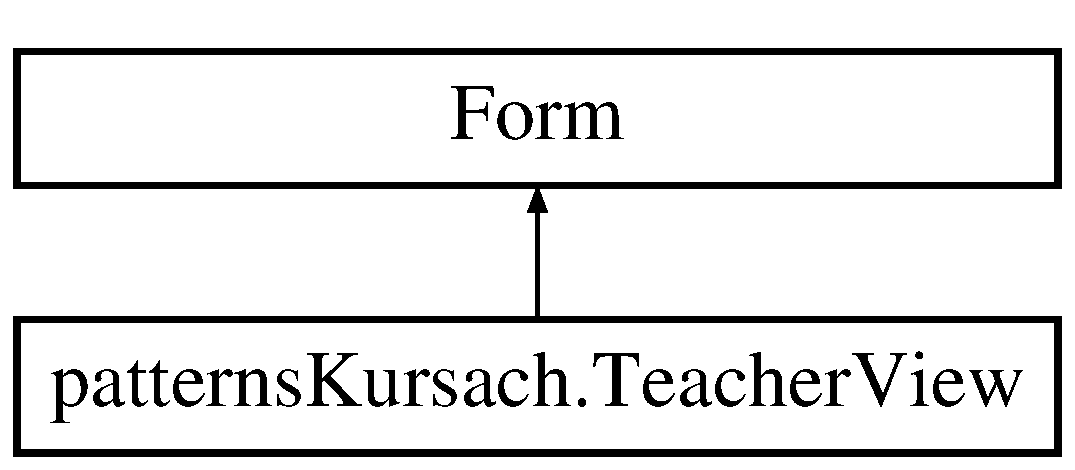
\includegraphics[height=2.000000cm]{classpatterns_kursach_1_1_teacher_view}
\end{center}
\end{figure}
\subsection*{Public Member Functions}
\begin{DoxyCompactItemize}
\item 
\mbox{\hyperlink{classpatterns_kursach_1_1_teacher_view_a1096d03ed22a60d848473f3a10f01179}{Teacher\+View}} ()
\item 
void \mbox{\hyperlink{classpatterns_kursach_1_1_teacher_view_aa56a700da1d0c37ca75abe74eb466b92}{Fill\+Teacher}} ()
\item 
void \mbox{\hyperlink{classpatterns_kursach_1_1_teacher_view_a2ab40a41ea53ff51d414a0baa237ec4b}{Fill\+Publish}} (int id)
\item 
void \mbox{\hyperlink{classpatterns_kursach_1_1_teacher_view_a3a143c68f1bdb8540beb11f023a969dc}{Fill\+Method}} (int id)
\end{DoxyCompactItemize}
\subsection*{Protected Member Functions}
\begin{DoxyCompactItemize}
\item 
override void \mbox{\hyperlink{classpatterns_kursach_1_1_teacher_view_a3c824cb6726bdf46cdb2b3de0578d4d9}{Dispose}} (bool disposing)
\begin{DoxyCompactList}\small\item\em Clean up any resources being used. \end{DoxyCompactList}\end{DoxyCompactItemize}


\subsection{Detailed Description}


Definition at line 14 of file Teacher\+View.\+cs.



\subsection{Constructor \& Destructor Documentation}
\mbox{\Hypertarget{classpatterns_kursach_1_1_teacher_view_a1096d03ed22a60d848473f3a10f01179}\label{classpatterns_kursach_1_1_teacher_view_a1096d03ed22a60d848473f3a10f01179}} 
\index{patterns\+Kursach\+::\+Teacher\+View@{patterns\+Kursach\+::\+Teacher\+View}!Teacher\+View@{Teacher\+View}}
\index{Teacher\+View@{Teacher\+View}!patterns\+Kursach\+::\+Teacher\+View@{patterns\+Kursach\+::\+Teacher\+View}}
\subsubsection{\texorpdfstring{Teacher\+View()}{TeacherView()}}
{\footnotesize\ttfamily patterns\+Kursach.\+Teacher\+View.\+Teacher\+View (\begin{DoxyParamCaption}{ }\end{DoxyParamCaption})}



Definition at line 18 of file Teacher\+View.\+cs.



\subsection{Member Function Documentation}
\mbox{\Hypertarget{classpatterns_kursach_1_1_teacher_view_a3c824cb6726bdf46cdb2b3de0578d4d9}\label{classpatterns_kursach_1_1_teacher_view_a3c824cb6726bdf46cdb2b3de0578d4d9}} 
\index{patterns\+Kursach\+::\+Teacher\+View@{patterns\+Kursach\+::\+Teacher\+View}!Dispose@{Dispose}}
\index{Dispose@{Dispose}!patterns\+Kursach\+::\+Teacher\+View@{patterns\+Kursach\+::\+Teacher\+View}}
\subsubsection{\texorpdfstring{Dispose()}{Dispose()}}
{\footnotesize\ttfamily override void patterns\+Kursach.\+Teacher\+View.\+Dispose (\begin{DoxyParamCaption}\item[{bool}]{disposing }\end{DoxyParamCaption})\hspace{0.3cm}{\ttfamily [protected]}}



Clean up any resources being used. 


\begin{DoxyParams}{Parameters}
{\em disposing} & true if managed resources should be disposed; otherwise, false.\\
\hline
\end{DoxyParams}


Definition at line 14 of file Teacher\+View.\+Designer.\+cs.

\mbox{\Hypertarget{classpatterns_kursach_1_1_teacher_view_a3a143c68f1bdb8540beb11f023a969dc}\label{classpatterns_kursach_1_1_teacher_view_a3a143c68f1bdb8540beb11f023a969dc}} 
\index{patterns\+Kursach\+::\+Teacher\+View@{patterns\+Kursach\+::\+Teacher\+View}!Fill\+Method@{Fill\+Method}}
\index{Fill\+Method@{Fill\+Method}!patterns\+Kursach\+::\+Teacher\+View@{patterns\+Kursach\+::\+Teacher\+View}}
\subsubsection{\texorpdfstring{Fill\+Method()}{FillMethod()}}
{\footnotesize\ttfamily void patterns\+Kursach.\+Teacher\+View.\+Fill\+Method (\begin{DoxyParamCaption}\item[{int}]{id }\end{DoxyParamCaption})}



Definition at line 62 of file Teacher\+View.\+cs.

\mbox{\Hypertarget{classpatterns_kursach_1_1_teacher_view_a2ab40a41ea53ff51d414a0baa237ec4b}\label{classpatterns_kursach_1_1_teacher_view_a2ab40a41ea53ff51d414a0baa237ec4b}} 
\index{patterns\+Kursach\+::\+Teacher\+View@{patterns\+Kursach\+::\+Teacher\+View}!Fill\+Publish@{Fill\+Publish}}
\index{Fill\+Publish@{Fill\+Publish}!patterns\+Kursach\+::\+Teacher\+View@{patterns\+Kursach\+::\+Teacher\+View}}
\subsubsection{\texorpdfstring{Fill\+Publish()}{FillPublish()}}
{\footnotesize\ttfamily void patterns\+Kursach.\+Teacher\+View.\+Fill\+Publish (\begin{DoxyParamCaption}\item[{int}]{id }\end{DoxyParamCaption})}



Definition at line 47 of file Teacher\+View.\+cs.

\mbox{\Hypertarget{classpatterns_kursach_1_1_teacher_view_aa56a700da1d0c37ca75abe74eb466b92}\label{classpatterns_kursach_1_1_teacher_view_aa56a700da1d0c37ca75abe74eb466b92}} 
\index{patterns\+Kursach\+::\+Teacher\+View@{patterns\+Kursach\+::\+Teacher\+View}!Fill\+Teacher@{Fill\+Teacher}}
\index{Fill\+Teacher@{Fill\+Teacher}!patterns\+Kursach\+::\+Teacher\+View@{patterns\+Kursach\+::\+Teacher\+View}}
\subsubsection{\texorpdfstring{Fill\+Teacher()}{FillTeacher()}}
{\footnotesize\ttfamily void patterns\+Kursach.\+Teacher\+View.\+Fill\+Teacher (\begin{DoxyParamCaption}{ }\end{DoxyParamCaption})}



Definition at line 31 of file Teacher\+View.\+cs.



The documentation for this class was generated from the following files\+:\begin{DoxyCompactItemize}
\item 
patterns\+Kursach/\mbox{\hyperlink{_teacher_view_8cs}{Teacher\+View.\+cs}}\item 
patterns\+Kursach/\mbox{\hyperlink{_teacher_view_8_designer_8cs}{Teacher\+View.\+Designer.\+cs}}\end{DoxyCompactItemize}

\hypertarget{classpatterns_kursach_1_1_work}{}\section{patterns\+Kursach.\+Work Class Reference}
\label{classpatterns_kursach_1_1_work}\index{patterns\+Kursach.\+Work@{patterns\+Kursach.\+Work}}
\subsection*{Public Member Functions}
\begin{DoxyCompactItemize}
\item 
\mbox{\hyperlink{classpatterns_kursach_1_1_work_a048e29adb18238c639ad66f68e016c49}{Work}} (int id, string name, string kind)
\item 
\mbox{\hyperlink{classpatterns_kursach_1_1_work_a8a6f1bcd6608b89d8a7e33b170492fc3}{Work}} (Data\+Row datas)
\end{DoxyCompactItemize}
\subsection*{Properties}
\begin{DoxyCompactItemize}
\item 
int \mbox{\hyperlink{classpatterns_kursach_1_1_work_a2ef9dc5b4453ca418818c10ddc609186}{Id}}\hspace{0.3cm}{\ttfamily  \mbox{[}get, set\mbox{]}}
\item 
string \mbox{\hyperlink{classpatterns_kursach_1_1_work_af3706083bb585a0cf3b6a69cddf9c45f}{Name}}\hspace{0.3cm}{\ttfamily  \mbox{[}get, set\mbox{]}}
\item 
string \mbox{\hyperlink{classpatterns_kursach_1_1_work_a40621d3042128256f9d180095fba721a}{Kind}}\hspace{0.3cm}{\ttfamily  \mbox{[}get, set\mbox{]}}
\end{DoxyCompactItemize}


\subsection{Detailed Description}


Definition at line 10 of file Work.\+cs.



\subsection{Constructor \& Destructor Documentation}
\mbox{\Hypertarget{classpatterns_kursach_1_1_work_a048e29adb18238c639ad66f68e016c49}\label{classpatterns_kursach_1_1_work_a048e29adb18238c639ad66f68e016c49}} 
\index{patterns\+Kursach\+::\+Work@{patterns\+Kursach\+::\+Work}!Work@{Work}}
\index{Work@{Work}!patterns\+Kursach\+::\+Work@{patterns\+Kursach\+::\+Work}}
\subsubsection{\texorpdfstring{Work()}{Work()}\hspace{0.1cm}{\footnotesize\ttfamily [1/2]}}
{\footnotesize\ttfamily patterns\+Kursach.\+Work.\+Work (\begin{DoxyParamCaption}\item[{int}]{id,  }\item[{string}]{name,  }\item[{string}]{kind }\end{DoxyParamCaption})}



Definition at line 18 of file Work.\+cs.

\mbox{\Hypertarget{classpatterns_kursach_1_1_work_a8a6f1bcd6608b89d8a7e33b170492fc3}\label{classpatterns_kursach_1_1_work_a8a6f1bcd6608b89d8a7e33b170492fc3}} 
\index{patterns\+Kursach\+::\+Work@{patterns\+Kursach\+::\+Work}!Work@{Work}}
\index{Work@{Work}!patterns\+Kursach\+::\+Work@{patterns\+Kursach\+::\+Work}}
\subsubsection{\texorpdfstring{Work()}{Work()}\hspace{0.1cm}{\footnotesize\ttfamily [2/2]}}
{\footnotesize\ttfamily patterns\+Kursach.\+Work.\+Work (\begin{DoxyParamCaption}\item[{Data\+Row}]{datas }\end{DoxyParamCaption})}



Definition at line 29 of file Work.\+cs.



\subsection{Property Documentation}
\mbox{\Hypertarget{classpatterns_kursach_1_1_work_a2ef9dc5b4453ca418818c10ddc609186}\label{classpatterns_kursach_1_1_work_a2ef9dc5b4453ca418818c10ddc609186}} 
\index{patterns\+Kursach\+::\+Work@{patterns\+Kursach\+::\+Work}!Id@{Id}}
\index{Id@{Id}!patterns\+Kursach\+::\+Work@{patterns\+Kursach\+::\+Work}}
\subsubsection{\texorpdfstring{Id}{Id}}
{\footnotesize\ttfamily int patterns\+Kursach.\+Work.\+Id\hspace{0.3cm}{\ttfamily [get]}, {\ttfamily [set]}}



Definition at line 25 of file Work.\+cs.

\mbox{\Hypertarget{classpatterns_kursach_1_1_work_a40621d3042128256f9d180095fba721a}\label{classpatterns_kursach_1_1_work_a40621d3042128256f9d180095fba721a}} 
\index{patterns\+Kursach\+::\+Work@{patterns\+Kursach\+::\+Work}!Kind@{Kind}}
\index{Kind@{Kind}!patterns\+Kursach\+::\+Work@{patterns\+Kursach\+::\+Work}}
\subsubsection{\texorpdfstring{Kind}{Kind}}
{\footnotesize\ttfamily string patterns\+Kursach.\+Work.\+Kind\hspace{0.3cm}{\ttfamily [get]}, {\ttfamily [set]}}



Definition at line 27 of file Work.\+cs.

\mbox{\Hypertarget{classpatterns_kursach_1_1_work_af3706083bb585a0cf3b6a69cddf9c45f}\label{classpatterns_kursach_1_1_work_af3706083bb585a0cf3b6a69cddf9c45f}} 
\index{patterns\+Kursach\+::\+Work@{patterns\+Kursach\+::\+Work}!Name@{Name}}
\index{Name@{Name}!patterns\+Kursach\+::\+Work@{patterns\+Kursach\+::\+Work}}
\subsubsection{\texorpdfstring{Name}{Name}}
{\footnotesize\ttfamily string patterns\+Kursach.\+Work.\+Name\hspace{0.3cm}{\ttfamily [get]}, {\ttfamily [set]}}



Definition at line 26 of file Work.\+cs.



The documentation for this class was generated from the following file\+:\begin{DoxyCompactItemize}
\item 
patterns\+Kursach/\mbox{\hyperlink{_work_8cs}{Work.\+cs}}\end{DoxyCompactItemize}

\chapter{File Documentation}
\hypertarget{_attestation_8cs}{}\section{patterns\+Kursach/\+Attestation.cs File Reference}
\label{_attestation_8cs}\index{patterns\+Kursach/\+Attestation.\+cs@{patterns\+Kursach/\+Attestation.\+cs}}
\subsection*{Classes}
\begin{DoxyCompactItemize}
\item 
class \mbox{\hyperlink{classpatterns_kursach_1_1_attestation}{patterns\+Kursach.\+Attestation}}
\end{DoxyCompactItemize}
\subsection*{Namespaces}
\begin{DoxyCompactItemize}
\item 
namespace \mbox{\hyperlink{namespacepatterns_kursach}{patterns\+Kursach}}
\end{DoxyCompactItemize}

\hypertarget{_db_connection_8cs}{}\section{patterns\+Kursach/\+Db\+Connection.cs File Reference}
\label{_db_connection_8cs}\index{patterns\+Kursach/\+Db\+Connection.\+cs@{patterns\+Kursach/\+Db\+Connection.\+cs}}
\subsection*{Classes}
\begin{DoxyCompactItemize}
\item 
class \mbox{\hyperlink{classpatterns_kursach_1_1_db_connection}{patterns\+Kursach.\+Db\+Connection}}
\end{DoxyCompactItemize}
\subsection*{Namespaces}
\begin{DoxyCompactItemize}
\item 
namespace \mbox{\hyperlink{namespacepatterns_kursach}{patterns\+Kursach}}
\end{DoxyCompactItemize}

\hypertarget{_i_store_adapter_8cs}{}\section{patterns\+Kursach/\+I\+Store\+Adapter.cs File Reference}
\label{_i_store_adapter_8cs}\index{patterns\+Kursach/\+I\+Store\+Adapter.\+cs@{patterns\+Kursach/\+I\+Store\+Adapter.\+cs}}
\subsection*{Classes}
\begin{DoxyCompactItemize}
\item 
interface \mbox{\hyperlink{interfacepatterns_kursach_1_1adapter_1_1_i_store_adapter}{patterns\+Kursach.\+adapter.\+I\+Store\+Adapter}}
\end{DoxyCompactItemize}
\subsection*{Namespaces}
\begin{DoxyCompactItemize}
\item 
namespace \mbox{\hyperlink{namespacepatterns_kursach_1_1adapter}{patterns\+Kursach.\+adapter}}
\end{DoxyCompactItemize}

\hypertarget{_login_8cs}{}\section{patterns\+Kursach/\+Login.cs File Reference}
\label{_login_8cs}\index{patterns\+Kursach/\+Login.\+cs@{patterns\+Kursach/\+Login.\+cs}}
\subsection*{Classes}
\begin{DoxyCompactItemize}
\item 
class \mbox{\hyperlink{classpatterns_kursach_1_1_login}{patterns\+Kursach.\+Login}}
\end{DoxyCompactItemize}
\subsection*{Namespaces}
\begin{DoxyCompactItemize}
\item 
namespace \mbox{\hyperlink{namespacepatterns_kursach}{patterns\+Kursach}}
\end{DoxyCompactItemize}

\hypertarget{_login_8_designer_8cs}{}\section{patterns\+Kursach/\+Login.Designer.\+cs File Reference}
\label{_login_8_designer_8cs}\index{patterns\+Kursach/\+Login.\+Designer.\+cs@{patterns\+Kursach/\+Login.\+Designer.\+cs}}
\subsection*{Classes}
\begin{DoxyCompactItemize}
\item 
class \mbox{\hyperlink{classpatterns_kursach_1_1_login}{patterns\+Kursach.\+Login}}
\end{DoxyCompactItemize}
\subsection*{Namespaces}
\begin{DoxyCompactItemize}
\item 
namespace \mbox{\hyperlink{namespacepatterns_kursach}{patterns\+Kursach}}
\end{DoxyCompactItemize}

\hypertarget{_metodichka_8cs}{}\section{patterns\+Kursach/\+Metodichka.cs File Reference}
\label{_metodichka_8cs}\index{patterns\+Kursach/\+Metodichka.\+cs@{patterns\+Kursach/\+Metodichka.\+cs}}
\subsection*{Classes}
\begin{DoxyCompactItemize}
\item 
class \mbox{\hyperlink{classpatterns_kursach_1_1_metodichka}{patterns\+Kursach.\+Metodichka}}
\end{DoxyCompactItemize}
\subsection*{Namespaces}
\begin{DoxyCompactItemize}
\item 
namespace \mbox{\hyperlink{namespacepatterns_kursach}{patterns\+Kursach}}
\end{DoxyCompactItemize}

\hypertarget{_program_8cs}{}\section{patterns\+Kursach/\+Program.cs File Reference}
\label{_program_8cs}\index{patterns\+Kursach/\+Program.\+cs@{patterns\+Kursach/\+Program.\+cs}}
\subsection*{Classes}
\begin{DoxyCompactItemize}
\item 
class {\bfseries patterns\+Kursach.\+Program}
\end{DoxyCompactItemize}
\subsection*{Namespaces}
\begin{DoxyCompactItemize}
\item 
namespace \mbox{\hyperlink{namespacepatterns_kursach}{patterns\+Kursach}}
\end{DoxyCompactItemize}

\hypertarget{_progress_8cs}{}\section{patterns\+Kursach/\+Progress.cs File Reference}
\label{_progress_8cs}\index{patterns\+Kursach/\+Progress.\+cs@{patterns\+Kursach/\+Progress.\+cs}}
\subsection*{Classes}
\begin{DoxyCompactItemize}
\item 
class \mbox{\hyperlink{classpatterns_kursach_1_1_progress}{patterns\+Kursach.\+Progress}}
\end{DoxyCompactItemize}
\subsection*{Namespaces}
\begin{DoxyCompactItemize}
\item 
namespace \mbox{\hyperlink{namespacepatterns_kursach}{patterns\+Kursach}}
\end{DoxyCompactItemize}

\hypertarget{_publish_8cs}{}\section{patterns\+Kursach/\+Publish.cs File Reference}
\label{_publish_8cs}\index{patterns\+Kursach/\+Publish.\+cs@{patterns\+Kursach/\+Publish.\+cs}}
\subsection*{Classes}
\begin{DoxyCompactItemize}
\item 
class \mbox{\hyperlink{classpatterns_kursach_1_1_publish}{patterns\+Kursach.\+Publish}}
\end{DoxyCompactItemize}
\subsection*{Namespaces}
\begin{DoxyCompactItemize}
\item 
namespace \mbox{\hyperlink{namespacepatterns_kursach}{patterns\+Kursach}}
\end{DoxyCompactItemize}

\hypertarget{_storage_adapter_8cs}{}\section{patterns\+Kursach/\+Storage\+Adapter.cs File Reference}
\label{_storage_adapter_8cs}\index{patterns\+Kursach/\+Storage\+Adapter.\+cs@{patterns\+Kursach/\+Storage\+Adapter.\+cs}}
\subsection*{Classes}
\begin{DoxyCompactItemize}
\item 
class \mbox{\hyperlink{classpatterns_kursach_1_1_storage_adapter}{patterns\+Kursach.\+Storage\+Adapter}}
\end{DoxyCompactItemize}
\subsection*{Namespaces}
\begin{DoxyCompactItemize}
\item 
namespace \mbox{\hyperlink{namespacepatterns_kursach}{patterns\+Kursach}}
\end{DoxyCompactItemize}

\hypertarget{_student_8cs}{}\section{patterns\+Kursach/\+Student.cs File Reference}
\label{_student_8cs}\index{patterns\+Kursach/\+Student.\+cs@{patterns\+Kursach/\+Student.\+cs}}
\subsection*{Classes}
\begin{DoxyCompactItemize}
\item 
class \mbox{\hyperlink{classpatterns_kursach_1_1_student}{patterns\+Kursach.\+Student}}
\end{DoxyCompactItemize}
\subsection*{Namespaces}
\begin{DoxyCompactItemize}
\item 
namespace \mbox{\hyperlink{namespacepatterns_kursach}{patterns\+Kursach}}
\end{DoxyCompactItemize}

\hypertarget{_student_mapper_8cs}{}\section{patterns\+Kursach/\+Student\+Mapper.cs File Reference}
\label{_student_mapper_8cs}\index{patterns\+Kursach/\+Student\+Mapper.\+cs@{patterns\+Kursach/\+Student\+Mapper.\+cs}}
\subsection*{Classes}
\begin{DoxyCompactItemize}
\item 
class \mbox{\hyperlink{classpatterns_kursach_1_1data_mapper_1_1_student_mapper}{patterns\+Kursach.\+data\+Mapper.\+Student\+Mapper}}
\end{DoxyCompactItemize}
\subsection*{Namespaces}
\begin{DoxyCompactItemize}
\item 
namespace \mbox{\hyperlink{namespacepatterns_kursach_1_1data_mapper}{patterns\+Kursach.\+data\+Mapper}}
\end{DoxyCompactItemize}

\hypertarget{_student_view_8cs}{}\section{patterns\+Kursach/\+Student\+View.cs File Reference}
\label{_student_view_8cs}\index{patterns\+Kursach/\+Student\+View.\+cs@{patterns\+Kursach/\+Student\+View.\+cs}}
\subsection*{Classes}
\begin{DoxyCompactItemize}
\item 
class \mbox{\hyperlink{classpatterns_kursach_1_1student}{patterns\+Kursach.\+student}}
\end{DoxyCompactItemize}
\subsection*{Namespaces}
\begin{DoxyCompactItemize}
\item 
namespace \mbox{\hyperlink{namespacepatterns_kursach}{patterns\+Kursach}}
\end{DoxyCompactItemize}

\hypertarget{_student_view_8_designer_8cs}{}\section{patterns\+Kursach/\+Student\+View.Designer.\+cs File Reference}
\label{_student_view_8_designer_8cs}\index{patterns\+Kursach/\+Student\+View.\+Designer.\+cs@{patterns\+Kursach/\+Student\+View.\+Designer.\+cs}}
\subsection*{Classes}
\begin{DoxyCompactItemize}
\item 
class \mbox{\hyperlink{classpatterns_kursach_1_1student}{patterns\+Kursach.\+student}}
\end{DoxyCompactItemize}
\subsection*{Namespaces}
\begin{DoxyCompactItemize}
\item 
namespace \mbox{\hyperlink{namespacepatterns_kursach}{patterns\+Kursach}}
\end{DoxyCompactItemize}

\hypertarget{_teacher_8cs}{}\section{patterns\+Kursach/\+Teacher.cs File Reference}
\label{_teacher_8cs}\index{patterns\+Kursach/\+Teacher.\+cs@{patterns\+Kursach/\+Teacher.\+cs}}
\subsection*{Classes}
\begin{DoxyCompactItemize}
\item 
class \mbox{\hyperlink{classpatterns_kursach_1_1_teacher}{patterns\+Kursach.\+Teacher}}
\end{DoxyCompactItemize}
\subsection*{Namespaces}
\begin{DoxyCompactItemize}
\item 
namespace \mbox{\hyperlink{namespacepatterns_kursach}{patterns\+Kursach}}
\end{DoxyCompactItemize}

\hypertarget{_teacher_mapper_8cs}{}\section{patterns\+Kursach/\+Teacher\+Mapper.cs File Reference}
\label{_teacher_mapper_8cs}\index{patterns\+Kursach/\+Teacher\+Mapper.\+cs@{patterns\+Kursach/\+Teacher\+Mapper.\+cs}}
\subsection*{Classes}
\begin{DoxyCompactItemize}
\item 
class \mbox{\hyperlink{classpatterns_kursach_1_1data_mapper_1_1_teacher_mapper}{patterns\+Kursach.\+data\+Mapper.\+Teacher\+Mapper}}
\end{DoxyCompactItemize}
\subsection*{Namespaces}
\begin{DoxyCompactItemize}
\item 
namespace \mbox{\hyperlink{namespacepatterns_kursach_1_1data_mapper}{patterns\+Kursach.\+data\+Mapper}}
\end{DoxyCompactItemize}

\hypertarget{_teacher_view_8cs}{}\section{patterns\+Kursach/\+Teacher\+View.cs File Reference}
\label{_teacher_view_8cs}\index{patterns\+Kursach/\+Teacher\+View.\+cs@{patterns\+Kursach/\+Teacher\+View.\+cs}}
\subsection*{Classes}
\begin{DoxyCompactItemize}
\item 
class \mbox{\hyperlink{classpatterns_kursach_1_1_teacher_view}{patterns\+Kursach.\+Teacher\+View}}
\end{DoxyCompactItemize}
\subsection*{Namespaces}
\begin{DoxyCompactItemize}
\item 
namespace \mbox{\hyperlink{namespacepatterns_kursach}{patterns\+Kursach}}
\end{DoxyCompactItemize}

\hypertarget{_teacher_view_8_designer_8cs}{}\section{patterns\+Kursach/\+Teacher\+View.Designer.\+cs File Reference}
\label{_teacher_view_8_designer_8cs}\index{patterns\+Kursach/\+Teacher\+View.\+Designer.\+cs@{patterns\+Kursach/\+Teacher\+View.\+Designer.\+cs}}
\subsection*{Classes}
\begin{DoxyCompactItemize}
\item 
class \mbox{\hyperlink{classpatterns_kursach_1_1_teacher_view}{patterns\+Kursach.\+Teacher\+View}}
\end{DoxyCompactItemize}
\subsection*{Namespaces}
\begin{DoxyCompactItemize}
\item 
namespace \mbox{\hyperlink{namespacepatterns_kursach}{patterns\+Kursach}}
\end{DoxyCompactItemize}

\hypertarget{_work_8cs}{}\section{patterns\+Kursach/\+Work.cs File Reference}
\label{_work_8cs}\index{patterns\+Kursach/\+Work.\+cs@{patterns\+Kursach/\+Work.\+cs}}
\subsection*{Classes}
\begin{DoxyCompactItemize}
\item 
class \mbox{\hyperlink{classpatterns_kursach_1_1_work}{patterns\+Kursach.\+Work}}
\end{DoxyCompactItemize}
\subsection*{Namespaces}
\begin{DoxyCompactItemize}
\item 
namespace \mbox{\hyperlink{namespacepatterns_kursach}{patterns\+Kursach}}
\end{DoxyCompactItemize}

%--- End generated contents ---

% Index
\backmatter
\newpage
\phantomsection
\clearemptydoublepage
\addcontentsline{toc}{chapter}{Index}
\printindex

\end{document}
